\documentclass[nofilelist,dvipsnames]{cslthse-msc}
% to show a list of used packages at the end of the document, delete the nofilelist option
%\documentclass{cslthse-msc}
%\setlength{\textfloatsep}{1pt plus 1.0pt minus 2.0pt}
\usepackage[utf8]{inputenc}
\usepackage[english]{babel}
\usepackage{amsmath}
\usepackage{amsthm}
\usepackage{graphicx}
\usepackage[titletoc, header, page]{appendix}
\usepackage{transparent}
\usepackage[
	backend=biber,
	style=numeric,
	sorting=none,
]{biblatex}
\addbibresource{report.bib}
%\setlength{\belowcaptionskip}{0pt}
\usepackage{parskip}
\usepackage{textcomp}
\usepackage{pdfpages}
\usepackage{enumitem}
\usepackage[export]{adjustbox}
\setlist[description]{leftmargin=1.5cm,labelindent=1cm}

% used to display the used files at the end. Select nofilelist as a package option to disable this
%\listfiles % initialize

%\geometry{showframe}
%better like this?
%\student{Flavius Gruian}{Flavius.Gruian@cs.lth.se}
\student{Stefan Eng}{atn08sen@lu.se}

\thesisnumber{LU-CS-EX: 2020-XX} % Birger Swahn will provide this number to you, once the thesis is ready for publication

\title{
  Usability testing on the web; Measuring how design impacts task performance
  times.
}
%\onelinetitle
%\twolinestitle
\threelinestitle
%\fourlinestitle

%\subtitle{A {\LaTeX} class}
\company{MASSIVE}
\supervisors{
  John Deer, \href{mailto:jdeer@company.com}{\texttt{jdeer@company.com}}
}{
  Don Jeer, \href{mailto:djeer@xy.lth.se}{\texttt{djeer@xy.lth.se}}
}
\examiner{Jane Doe, \href{mailto:jane.doe@cs.lth.se}{\texttt{jane.doe@cs.lth.se}}}

\date{\today}
%\date{January 16, 2015}

\acknowledgements{
}

\theabstract{
}

\keywords{
	Usability testing,
	Web-application,
	Flask,
	HTML
}

\begin{document}
\renewcommand{\bibname}{References}

%\makefrontmatter
\newcommand{\todo}[1]{\textcolor{blue}{\textbf{TODO:} #1}}
\newcommand{\todoMaybe}[1]{\textcolor{OliveGreen}{\textbf{?TODO:} #1?}}
\newcommand{\eatdot}[1]{}
\newcommand{\ctitle}[1]{\citetitle{#1}\cite{#1}}
\newcommand{\varHere}[1]{\input{vars/#1.txt}\unskip}
\newcommand{\checkTruth}[0]{\textcolor{red}{(?)}}%
\newcommand{\findref}[0]{\textcolor{orange}{[!]}}%
\newcommand{\todoInsert}[1]{\textcolor{purple}{\textit{<insert #1 here>}}}%
\newcommand{\numRuns}[1]{\texttt{\#r=#1}}%

\includepdf[pages=-]{preface.pdf}
\tableofcontents

\chapter{Introduction}

  As the gaming industry continue to grow{\findref\findref} so do the reported
  number of stress-related issues reported by the people working in the
  sector{\findref\findref\findref}. The initial idea for this report came from a managers
  observation that co-workers would abandon the digital communication software
  for a more hands-on approaches, such as post-it notes on a whiteboard, when
  the pressure got to a certain point.

  Asking why, people stated that the software they were supposed to use for
  communicating and propagating the projects status throughout the team got in
  their way. Which is why they opted to use post-it notes, even though it has
  significantly worse communication bandwidth and is less accessible,
  at-least-it-works\texttrademark.

  \section[MASSIVE Entertainment | A Ubisoft studio]{MASSIVE}

  {\vspace{-0.7cm}{\hspace{1.85cm}\small MASSIVE ENTERTAINMENT | A UBISOFT STUDIO}}

    \todo{Expand section.}

	\section{Report goals}

		\begin{enumerate}
			\item{Create a web based platform for usability testing.}
			\item{Run one or several interface tests with real users on the platform.}
			\item{
				Verify that the collected data shows a significant\checkTruth impact on the studied
				variable(s) when parameters are changed. \todoMaybe{Shorten}
			}
		\end{enumerate}


%  \section{Usability testing}
%
%    \subsection{State of the art}
%
%      \todo{Expand this section.}

%  \section{Running usability tests at larger scales}
%
%    \subsection{Notable usability tests}
%
%      \todo{See if there are any notable large-scale usability tests, does A/B
%        testing for large websites count?}

	\section{Literary scope}

		This report draws and builds on information from the fields of usability
		testing, web design and interaction design.

		Specifically, \ctitle{citeHandbookUsability} and
		\ctitle{citeUsabilityTestingEssentials}, provide a contrast between
		traditional and modern approaches to usability testing and how to perform
		them.

		\ctitle{citeDonMakeMeThink} provides a concise and interesting
		summary of no-nonsense approaches to web design from a usability perspective.
		Last but not least \ctitle{citeTheDesignOfEverydayThings} introduces
		both \textit{user-centered-} and \textit{interaction-design} together
		with the concept of \textit{affordances},

	  %Introduction to user interface design and usability testing? \\
	  %
		%Figure out how much of an impact different design aspects have on tasks
		%that require distinguishing one element from another. And doing it in a
		%decentralised manner based on web-application. \\
	  %
	  %Don't make me think -> webdesign. \\
	  %Design of everyday things -> webdesign. \\
	  %Report based on distances / colors -> webdesign. \\
	  %Usability-testing guide -> webapp suggesting + other. \\


%	\chapter{Approach}
	\chapter{Background theory}

    \section{Usability}

      \subsection{Why usability testing?}

        Initially, the plan was to make interface changes to the
        organization-software itself, but a question remained, how do you prove
        that it actually makes a difference?

        \todo{Describe why usability testing, add scaling problem.}

      \subsection{Introduction}

        Usability is traditionally done in person with the \textit{over the
        shoulder} method which gives a good insight of what a participant does
        during a test. Further more, if the \textit{thinking out aloud -
        method} is utilized correctly, the test-moderator should have a good
        insight into the participant thought-process during the test.

      \subsection{Evolution and current use}

        While effective\checkTruth this method scales poorly with a one to one
        ratio between moderator and test participant. This project investigates
        the possibility of alleviating this scale constraint by utilizing a
        internet based platform to conduct usability tests of user interfaces
        online.

        \todo{Expand this section.}


    \section{Python}

    \section{Flask}

    \section{Scalable Vector Graphics}

    \section{To JavaScript or not to JavaScript}

	\chapter{Development process}

    The overall process took inspiration from agile software development with a
    touch of 'design-school'. \todo{Fix this section.}

    \begin{figure}[h!]
      \centering
      \includegraphics{figures/method.pdf}
      \caption{Concept, development, testing and improvement cycle.}
    \end{figure}

		\section{Brainstorming-sessions and interviews}{\label{label_sectionIdeas}

      In order to figure out a interesting approach, two brainstorming-sessions
      were conducted. The first in order to figure out what could be beneficial
      to the team and studio at large. Secondly, discussing possible academic
      applications and results.

      After hearing about the communication regression, it was decided that
      it would be interesting to see if there are certain design elements and
      theories that hold up better under stressful scenarios than others. A
      secondary goal included trying to make a testing platform 'from-scratch'
      in order to see if it would be feasible for a smaller research- or
      developer-team to conduct similar evaluations in-house on a small budget.

      To deicide what type of mock-assignments the tests should be constructed
      from, three in-person interviews were conducted. The managers were asked
      about what they would like to see implemented in order to make their
      day-to-day work easier, producing the following ideas:

      \newcommand{\ideaOne}{%
        An easy way to see if a co-worker is assigned more work than they have
        available hours.%
      }

      \newcommand{\ideaTwo}{%
        Calendar overview where it is possible to determine if there are
        hot-spots where lots of results need to be produced at the same
        time.%
      }

      \newcommand{\ideaThree}{%
        A concise way to identify if there are critical tasks that, if
        delayed, would delay other tasks that depend on it.%
      }

      \newcommand{\ideaFour}{%
        The possibility to identify a group or teams strengths and assign
        task types accordingly.%
      }

      \begin{itemize}
        \item{\ideaOne\label{label_ideas}}
        \item{\ideaTwo}
        \item{\ideaThree}
        \item{\ideaFour}
      \end{itemize}


		\section{Lo-fi prototypes}

      After taking some pointers from \findref, together with the suggestions
      gathered from the manager-interviews, four simple paper prototypes, shown
      below, were printed and presented to a second group of five interviewees
      for evaluation.

        \begin{figure}[h!]
          \center
          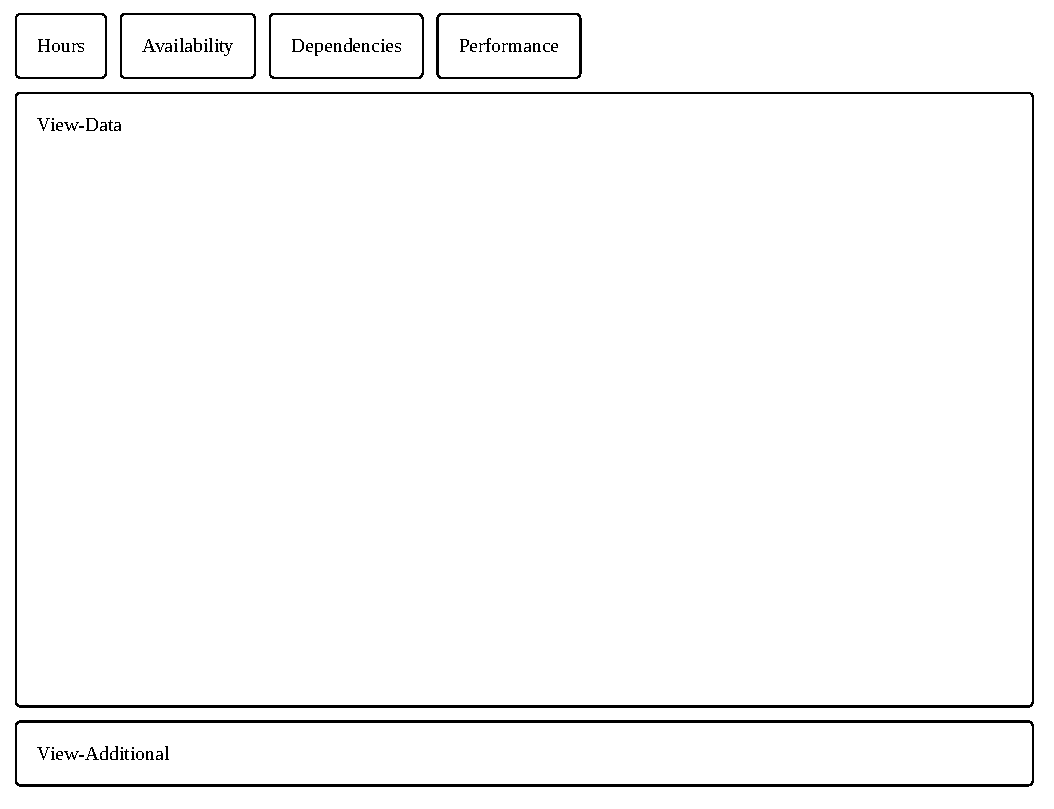
\includegraphics[valign=t,trim={.10cm .10cm .35cm .25cm},clip,width=.49\linewidth]{ui11.pdf}
          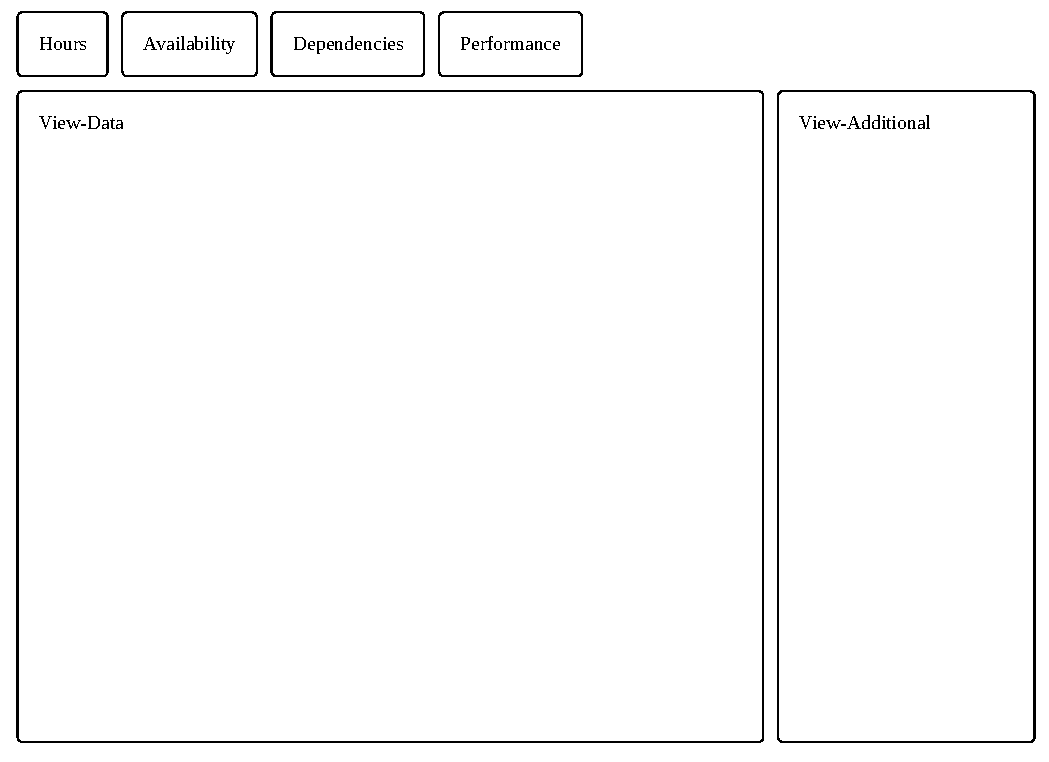
\includegraphics[valign=t,trim={.15cm .30cm .20cm .20cm},clip,width=.49\linewidth]{ui12.pdf}
          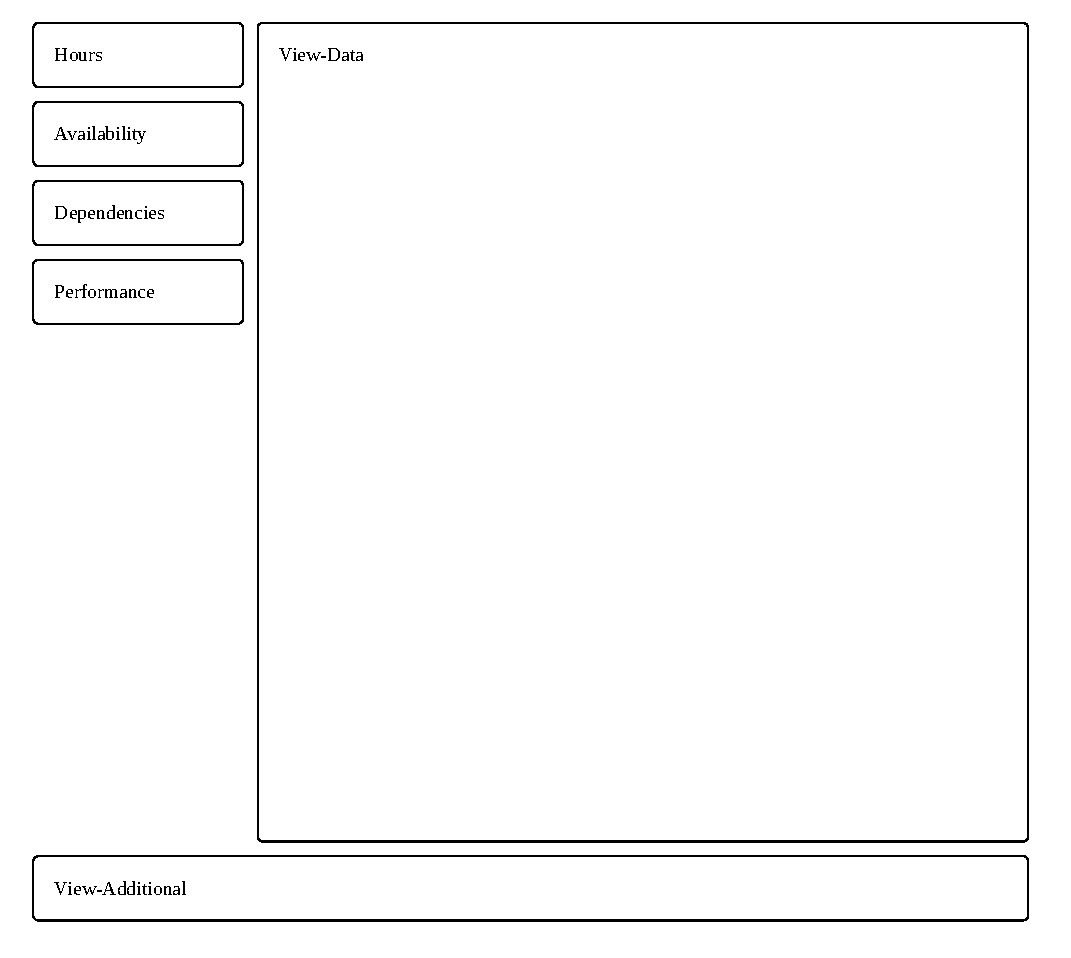
\includegraphics[valign=t,trim={.45cm .55cm .65cm .35cm},clip,width=.49\linewidth]{ui13.pdf}
          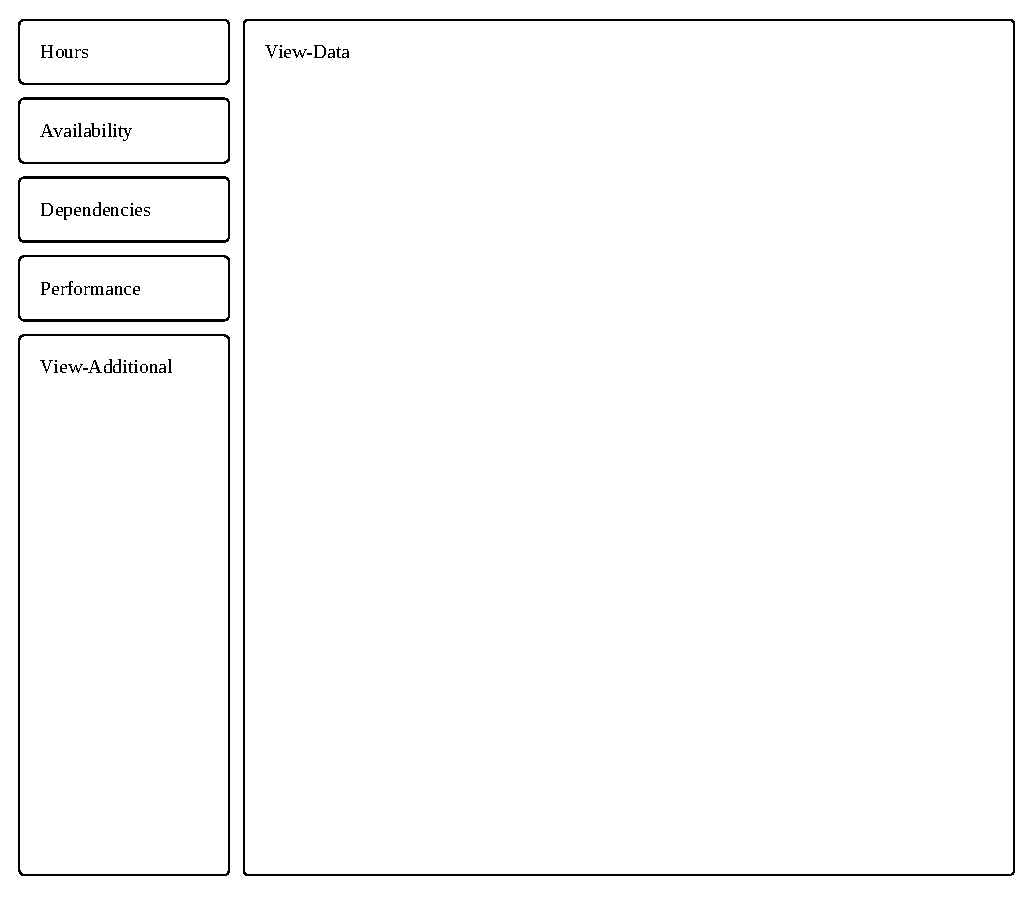
\includegraphics[valign=t,trim={.25cm .35cm .30cm .25cm},clip,width=.49\linewidth]{ui14.pdf}
          \caption{Interface drafts 1.1, 1.2, 1.3 and 1.4}
          \label{label_mockupInterfaces}
        \end{figure}

      The main difference is the placement of the main interface elements, with
      the first group having them on top, and the second one the left side.
      Lager versions of prototypes and itemized result from the interviews are
      found in \todoInsert{result link for interviews and larger prototypes.}

      \subsection{Interview structure for prototype selection}

        \begin{figure}[h!]
          \centering
          \includegraphics[trim={0 0 0 0},clip]{figures/lofi_method.pdf}
          \caption{Overall structure of prototype selection interviews.}
        \end{figure}

        These interviews were conducted in-person, with five team members, on
        the premises of Massive. The interview started with a description of
        what was happening; an evaluation of four different mock-up interfaces
        to determine which one was the most suitable for further testing.

        After confirming that there were no immediate questions, the
        interviewee was presented with the printed mockups in the same
        arrangement as shown in figure \ref{label_mockupInterfaces}. They were
        then asked to evaluate, out loud, the interfaces in any order they
        wished, and to ask if there was anything unclear about the assumed
        functionality.

        When the participant felt they were done and any questions they had
        about the interface were sorted out, they were asked to sort the
        prototypes from best- to least-suited for the upcoming test purpose.
        Again, the participant was asked to voice their thought process out
        aloud as they did the sorting.

        After confirming that the interviewee was satisfied with their
        ordering, a set of ten flash-cards were introduced. These cards
        represent the combined key-words-attributes from ISO 9241-11{\findref}
        and ISO 9241-12{\findref}, concerning usability and presentation of
        information respectively.

        Keyword definitions presented below:

            \begin{description}[style=nextline]
              \item[Effectiveness]{
                Usability is measured by the extend to which the
                intended goals of use of the overall system are achieved.
              }
              \item[Efficiency]{
                The resources that have to be expended to achieved the indented
                goals.
              }
              \item[Satisfaction]{
                The extent to which the user finds the overall system
                acceptable.
              }
              \item[Clarity]{
                  The information content is conveyed quickly and accurately.
              }
              \item[Discriminability]{
                  The displayed information can be distinguished
                  accurately.
              }
              \item[Conciseness]{
                  Users are not overloaded with extraneous information.
              }
              \item[Consistency]{
                  A unique design, conformity with user's expectation.
              }
              \item[Detectability]{
                  The user's attention is directed towards information
                  required.
              }
              \item[Legibility]{
                  Information is easy to read.
              }
              \item[Comprehensibility]{
                  The maning is clearly understandable, unambiguous,
                  interpretable, and recognizable.
              }
            \end{description}

        Where the top three terms are defined in ISO 9241-11 with the remainder
        coming from ISO 9241-12.

        The next task was for each participant to order the keywords
        in order of how important they thought that specific quality was for a
        well-functioning, user interfacing software. There were no restrictions
        in regards to the number of times a participant could ask about the
        definition or clarification of each term.

        When the participant acknowledged that they were finished with their
        selection, it was recorded, and the were asked to do one final task.
        Each participant was asked to re-evaluate their previously selected
        ranking of the prototype interfaces, changing the order if they felt
        another one was more appropriate after being exposed to the ISO
        definitions.

%        evaluation. The evaluation was conducted as an in-person interview
%        where the interviewee was asked to voiced their thoughts out aloud.
%        After the initial reaction and thought about each of the designs, the
%        interviewee was asked to pick, according to them, the most suitable
%        design.
%
%        After the initial pick, the interviewee was presented with
%        \todoInsert{part about ISO-standard design}, which they had to arrange
%        in order of most to least important according to their own views.
%        After prioritizing the different design attributes, the participant was
%        again asked to pick what they felt was the most suitable design.
%
%
%        \todo{Expand with information about ISO design standard}
%

    \section{Hi-fi prototype}

    After completing the interviews and tallying which paper prototype that
    was sorted first the most times, the result was paper prototype 1.4.

      \subsection{Input methods and screen sizes}

      \todo{Spell out the input alternatives} While the choices for the input
      method, except the last one, corresponds directly to a concrete input
      method used in human-computer interactions, the screen-sizes are somewhat
      ambiguous. This was an active choice in order to not alienate
      participants by forcing them to specify an actual measurement for the
      screen size. The assumed values for the screen-sizes ranges for the given
      choices are:
      \textit{Desktop} $>$17",
      \textit{Laptop}  12"-17",
      \textit{Tablet}  7"-12" and
      \textit{Mobile}  $<$7".




%		\section{Method}
%
%      This section expands on the methodology behind the initial concept and
%      creation of the testing platform, as well as the process of generating
%      and evaluating data from the usability tests performed by the participants.
%
%      \subsection{Software development methodology}
%
%        The goal was to adopt an agile development process{\findref} for the
%        creation, evaluation and improvement of the usability testing platform.
%
%        This methodology is centered around creating a minimal
%        working prototype{\findref} that is put in front of real users as soon
%        as possible. The feedback data generated by the users should then be
%        feed back into the design to improve the next prototype version, which
%        is tested again. This cycle should then be repeated until either the
%        software is satisfactory or the time is up.
%
%%      The goal was to perform several full iteration cycles, but in the
%%      end
%%      While this was the goal, it only completed one whole full cycle, with
%%      smaller iterations within the larger cycle. \todo{Reword}
%
%      \subsection{Defining the initial concept}
%
%        In order to perform usability tests that can be measured and validated,
%        there needs to something for users to interact with. Since the subject
%        of communication under pressure was the initial focus, the suggestion
%        of helping managers reduce the stress for their team came up.
%
%        After interviewing a few managers, the following ideas were
%        gathered:
%
%
%      \subsection{Paper prototypes for a first-draft interface}
%
%        Even though the initial interface setup was very bare-bones, it was
%        still important to get it in front of users, in this case, test
%        participants, as soon as possible.
%
%        %\begin{figure}[h!]
%        %  \centering
%        %  \begin{minipage}{.49\textwidth}
%        %    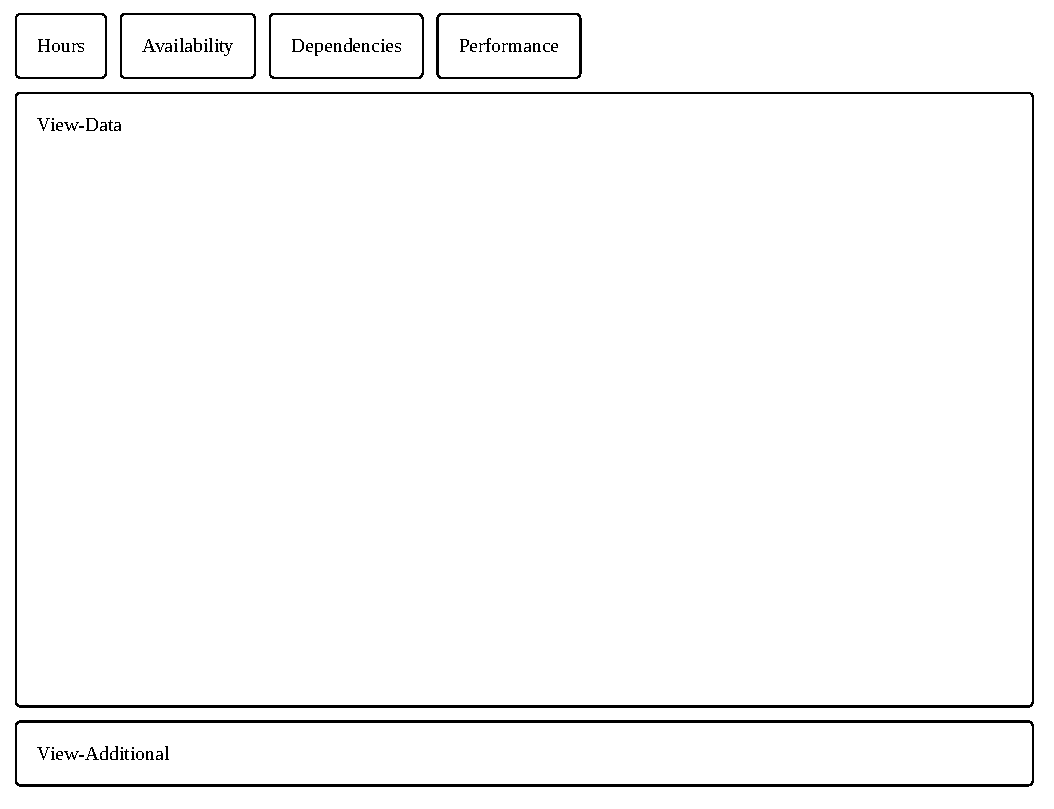
\includegraphics[width=\linewidth]{ui11.pdf}
%        %  \end{minipage}
%        %  \begin{minipage}{.49\textwidth}
%        %    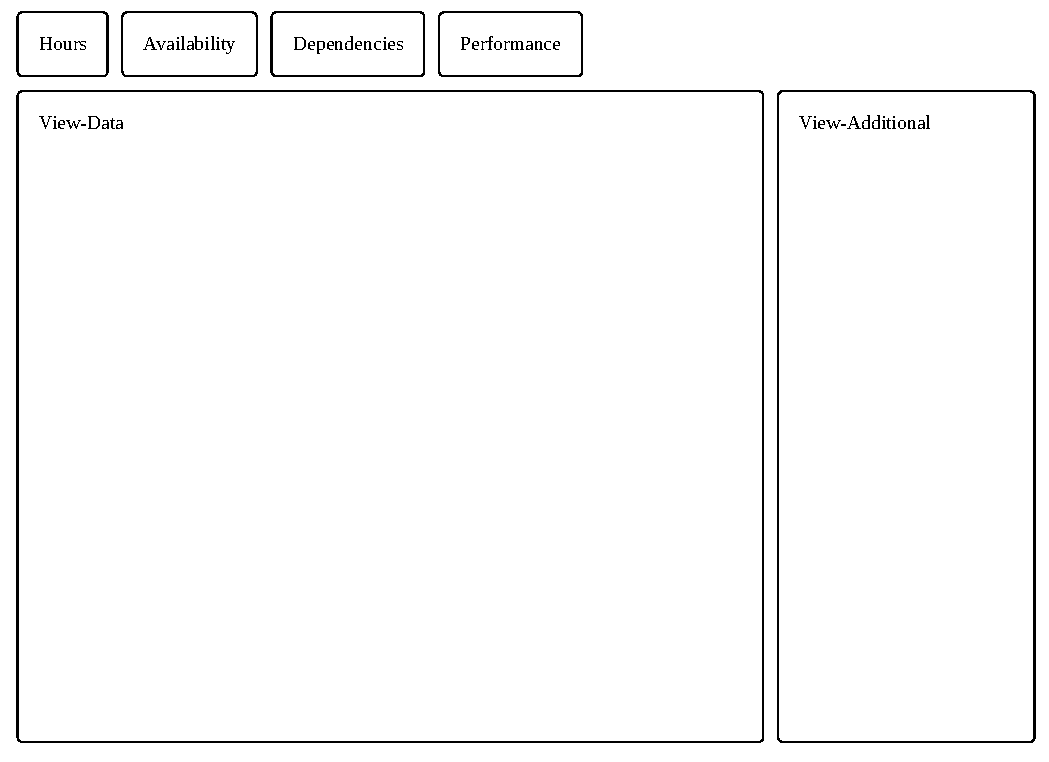
\includegraphics[width=\linewidth]{ui12.pdf}
%        %  \end{minipage}
%        %  \begin{minipage}{.49\textwidth}
%        %    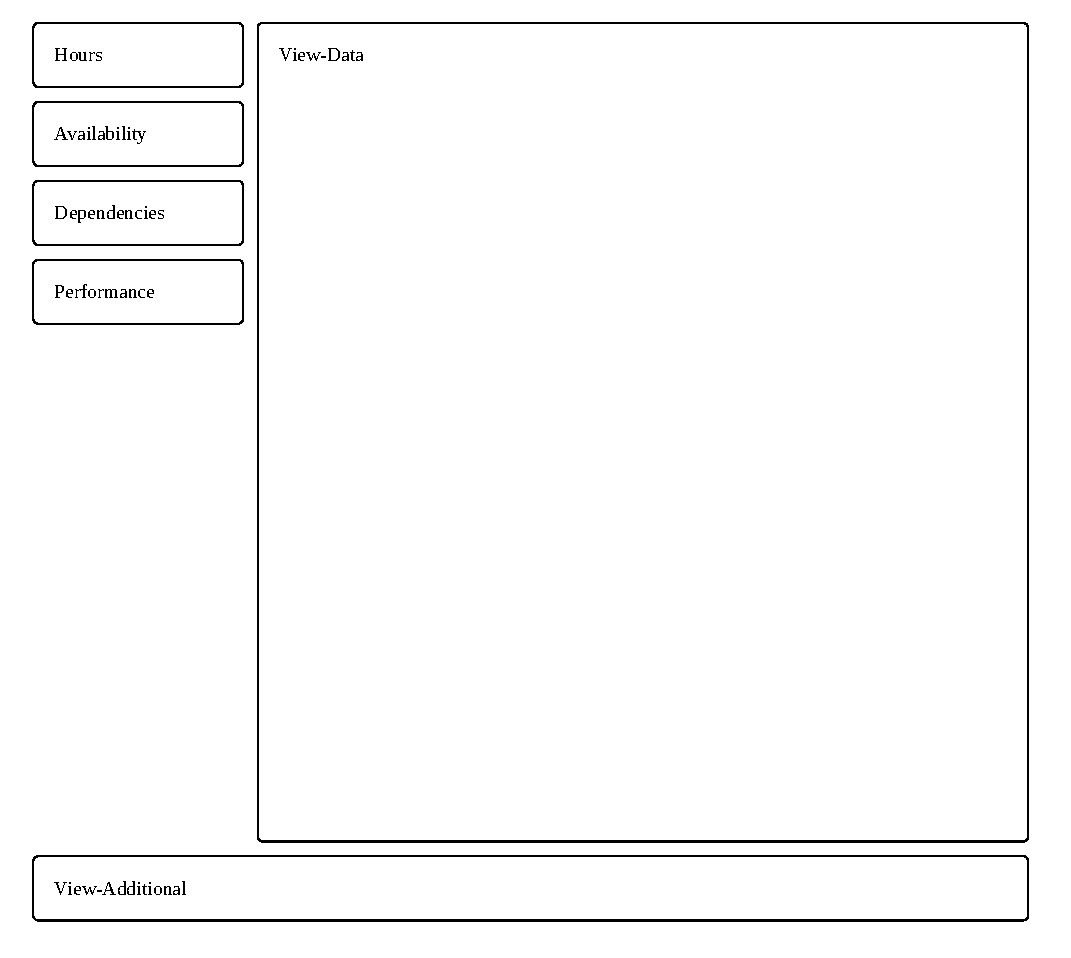
\includegraphics[width=\linewidth]{ui13.pdf}
%        %  \end{minipage}
%        %  \begin{minipage}{.49\textwidth}
%        %    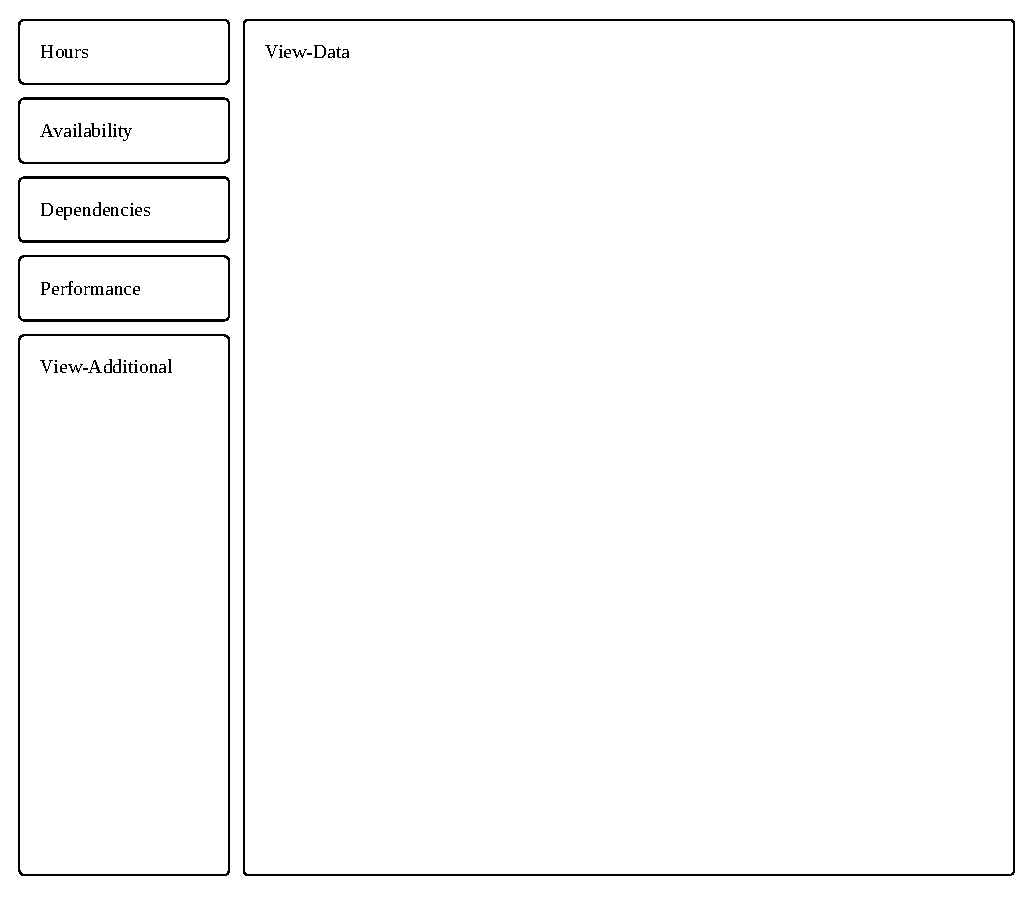
\includegraphics[width=\linewidth]{ui14.pdf}
%        %  \end{minipage}
%        %  \caption{Interface drafts 1.1, 1.2, 1.3 and 1.4.}
%        %\end{figure}
%
%        %\todoMaybe{These figures should probably be under result?}
%
%        Four mock-up interfaces were created based on \todoInsert{part about
%          ui design reference} and presented to five\checkTruth colleagues for
%        evaluation. The evaluation was conducted as an in-person interview
%        where the interviewee was asked to voiced their thoughts out aloud.
%        After the initial reaction and thought about each of the designs, the
%        interviewee was asked to pick, according to them, the most suitable
%        design.
%
%        After the initial pick, the interviewee was presented with
%        \todoInsert{part about ISO-standard design}, which they had to arrange
%        in order of most to least important according to their own views.
%        After prioritizing the different design attributes, the participant was
%        again asked to pick what they felt was the most suitable design.
%
%
%        \todo{Expand with information about ISO design standard}
%
%      \subsection{Gathering relevant test data}
%
%        There is a two-fold goal that the collected test-data needs to solve:
%        \begin{itemize}
%          \item{
%            Generate a quantifiable value that can be tracked in order to
%            evaluate the participants performance during tests.
%          }
%          \item{
%            Aggregate participant feedback about the platform in order to
%            improve the next version.
%          }
%        \end{itemize}
%
%        The first problem is solved by sticking with a established tradition
%        within usability testing\findref\findref, measuring completion time.
%        In order to keep track of their test-runs, participant are assigned an
%        anonymous id-string after acknowledging that they have read the initial
%        information. The anonymous id is registered as used in the database
%        and the id is stored in the participants browsers web-session.
%
%        As a participant starts a new task, the database will register the
%        start-time and link it to the aforementioned anonymous id. If the
%        participant completes the task, the stop-time will be recorded in the
%        same database post, and the difference between these two values will be
%        used as the time for task completion.
%
%        Acquiring feedback data is done through a post-test survey with ten set
%        questions (1-5) and a free-from dialog box for additional input.
%        \todo{Expand and reword last section}
%
%
%      \subsection{Evaluating impact and effectiveness}
%
%        First the test-measurements and feedback is recorded from the
%        participants and stored to the underlying database. This data can then
%        be processed in order to find interesting correlations between
%        different application variables, such as the test types impact on the
%        overall completion time.
%
%        The data is accumulated and processed using Python, specifically Python
%        3.8.1 as of the time of this writing. The graphs included in this paper
%        are generated through matplotlib, and numpy was used in select
%        instances.
%
%%        Since the data is stored in real-time and is available
%
%%			Results by measuring the time and showing graphs + statistical grouping /
%%			analysis.
%
%		\section{Theory}
%
%			\subsection{Information presentation and color}
%
%        This looks into the interaction between the Human Visual System (HVS)
%        and Graphical User Interfaces (GUIs), specifically the impact of color
%        on this interaction.
%
%        \todo{Expand section}
%
%			\subsection{Representative high fidelity prototypes}
%
%        User-Centered design and other iterative methods place a large
%        importance on creating a high fidelity prototyp\findref that users can interact
%        with, the sooner the better\findref.
%
%        In order to create a high fidelity prototype from the paper prototypes
%        presented earlier, each task had to be broken down into its essential
%        component. All the given examples given from the managers revolved
%        around identifying a specific piece of information, surrounded by
%        similar data in order to act on it.
%
%        \todo{Expand on 'finding a needle' approach with all the tasks, easy to
%        time and evaluate.}
%
%
%%			\subsection{Measuring time to task completion}
%%
%%
%%        \todo{Expand section}
%
%			\subsection{Thresholds for test failures}
%
%        Is there a clear limit to when a participant should no longer be able
%        to detect differences in color and relative sizes?
%
%        \todo{Expand section}
%
%
%		\section{Implementation}
%
%      This section specifies how the user-facing web-application and its
%      backend was constructed, and what the thought behind some of the
%      decisions were.
%
%%			Writing a web-application with Flask + python + sqlite3.
%%			HTML5 and CSS with a dab javascript.
%
%			\subsection{Platform software stack}
%
%        The main user interfacing application is written in Python together
%        with the Flask web-framework running on top of an Apache web-server.
%        On the backend sqlite3 is used in order to store the results and
%        feedback from participants for easy retrieval.
%
%        While trying to keep the amount of JavaScript to a minimum, in order to
%        have the highest possible interoperability rate, some snippets were
%        required in order to make it possible to submit a web-form by clicking
%        a SVG-graphic.
%
%			\subsection{Interface creation}
%
%        Interface wise the application is built in plain HTML5 markup to
%        organize the main structure and buttons. All the various interfaces for
%        the different tasks are constructed using Scalable Vector Graphics
%        (SVG).
%
%			\subsection{Variable challenges}
%
%        Randomness provides a good source of test-material but is not a good
%        fit for reproducibility. Fortunately this can be omitted by giving the
%        random number generator a pre-determined seed as a parameter to its
%        initialization call. Since the generator uses this seed as the basis
%        for all the random number sequences it produces, in other words, the
%        sequence of variables produced by two random number generators given
%        the same seed should be identical.
%
%        In this setup, the initial generator uses a hard-coded seed to to
%        produce a few thousand unique alpha-numeric sequences that are then
%        used as the anonymous ids for the participants. It is also these
%        anonymous-ids that are used as the seeds when generating the different
%        data-sets for each use.
%
%        This makes it possibility to reconstruct a participants test by
%        re-supplying the same anonymous-id and test-type to the application and
%        it should return the same test-setup.
%
%
%\addtocontents{toc}{\pagebreak}
	\chapter{Evaluation}

    After the test application was implemented and deployed, a link to the
    application was shared on the authors personal Facebook-profile together
    with an explanation of what the purpose of the test was. Three days
    later, the same link was shared on the Massive internal mailing list.

    \begin{figure}[h!]
      \centering
      \includegraphics{figures/deploy_link.pdf}
      \caption{Link-distribution and test milestones.}
      \label{label_milestones}
    \end{figure}

    Looking at the test setup and the final result, the participants can be
    grouped into three categories, depending how far through the test-session
    they ended up. The test structure has the following milestones:
    \begin{itemize}
      \item{Getting past the initial information and consent form.}
      \item{Completing the pre-survey.}
      \item{Completing the post-survey.}
    \end{itemize}

    \section{Basis and purpose of the test-tasks}

    The basis for the test-tasks is derived from the items displayed at the
    end of section \ref{label_sectionIdeas} at page \pageref{label_ideas}.
    This list contains a selected subset of the answers to the
    interview question of what tooling is currently missing that could make
    the day-to-day work for interviewed managers easier.

    Using these examples of what could feasibly be implemented to add
    real-world value to current day-to-day activities gives a concrete
    foundation to base the test-task design on. However, since all of
    the select suggestions could be implemented as a self-contained tool or
    service in their own right, implementing each of them fully, with
    correct behaviour, is outside the scope of this report.

    Due to the limited time and development resources mentioned above, each
    suggestion will be abstracted to its simplest goal that still contains
    the core function of the original. Since the overarching goal is to
    measure if the design of the test has any impacts on the performance,
    the main focus will be on tracking the time to completion of the task
    as accurately as possible.


	  \section{Participants}

    Out of the total of five days the application was live, in the first
    three days there were 27 participants that got past the first milestone,
    with 23 (85.2\%) of them completing the post-survey. At the third day a
    link to the application was shared internally at Massive. The final
    combined result over the five day span was; 101 participants getting past
    the initial information, 79 (78.2\%) answered the initial survey and a
    total of 74 (73.3\%) completing the post-survey.

    Since there is no concrete information to work with for users that only
    passed the first milestone, that group is excluded and the pre-survey and
    post-survey groups will receive further analysis.

      \subsection{Age, gender-identity and completion times}

      In the pre-post-survey group, the average age is, 30.5 years, 28
      participants (32.9\%) identify as female, 54 (63.5\%) as male and 3
      (3.5\%) as other. Looking at the post-survey group, the average age of
      the participants shifts slightly, 31.1 years, and 24 (32.4\%), 47
      (63.5\%) and 3 (4\%) of the participants identify as female, male and
      other respectively.

      Looking at completion times for the post-post-survey group, the average
      time from registration to finishing the last test-question was 20 minutes
      and 56 seconds with a median of 4 minutes and 23 seconds. Additionally,
      the fastest completion time was 37 seconds with the longest completion
      time clocking in at 14 hours 15 minutes and 35 seconds.

      \subsection{Prerequisites, prior knowledge and education}

      Other attributes that were deemed interested included; how comfortable
      the participant felt using a computer, if they hade any general interest
      in user interface design and if they had studied user interface design in
      any capacity. They were also questioned on if they regularly practiced
      precise mouse movements through games and similar activities and finally
      if they have trouble distinguishing colors from each other. These
      questions were posed as a personal statement, such as, ''\textit{I feel
        comfortable using a computer}'' together with a range of selectable
      numerical options, ranging from one, \textit{strongly disagree} to five,
      \textit{strongly agree}.

%      The initial Facebook link gathered 27 recorded test runs after three
%      days. After sharing the link to the test internally on Massive, an
%      additional 74 completions of the test were recorded over a span of two
%      days. In total, 101 completions, from pre- to post-questionnaire were
%      recorded over a five day span.
%
%
%      According to the pre-questionnaire, that the average age of a participant
%      is 30 years, .



%      Where from?
%
%      How many?
%
%      Section male / female / other.
%
%      Average arg.
%
%      Average test-session.
%
%
%      \section{Participants where from?}
%
%      \section{?}

    \section{Setup}

%      \begin{figure}[h!]
%        \centering
%        \includegraphics{figures/information_setup.pdf}
%        \caption{Information gathering process.}
%      \end{figure}

    \subsection{Dealing with varying testing hardware}

      Since the tests were done remotely via the internet, only requiring a
      device capable running a standard browser, there was no standardized
      hardware-setup that the tests were executed on. In order to have the
      possibility to analyze impact of different types of hardware and group
      different results, the pre-questionnaire included questions about what
      kind of hardware the participant was using to access the tests.

      It was concluded that screen size and input method had the largest
      probability to affect the result given the design of the tests.
      The participants were asked to specify their screen size by selecting one
      of the following options: \textit{desktop, laptop, tablet} or
      \textit{mobile}. As for the input method the choices were:
      \textit{mouse, trackpad, touch} or \textit{other}, see figure
      \ref{label_preSurvey} for a capture.

    \section{Procedure}

      \begin{figure}[h!]
        \centering
        \includegraphics{figures/test_flow.pdf}
        \caption{Illustrated flow for overall test-session.}
      \end{figure}

      \begin{figure}[h!]
        \centering
        \includegraphics{figures/test_flow_task_runs.pdf}
        \caption{Illustrated flow for individual task-runs.}
      \end{figure}

      \subsection{General information, consent and initial survey}

        When accessing the test the participant is greeted by a information and
        consent screen, detailing the goals of the test and how the information
        generated by their activity will be used. The page explains that this
        is a usability study, and though there will be information collected,
        anything that will be publicised will be aggregations and include no
        personally identifiable information. The full information and consent
        page can be found in figure \ref{label_infoConsent}.

        Participant that accept and submit the consent form are then navigated
        to the main landing page. This page acts as a hub for the duration of
        the test session, providing access to all other parts of testing
        application. On the first visit the main view of the landing page is
        occupied by the initial survey, shown below.

        \begin{figure}[h!]
          \centering
          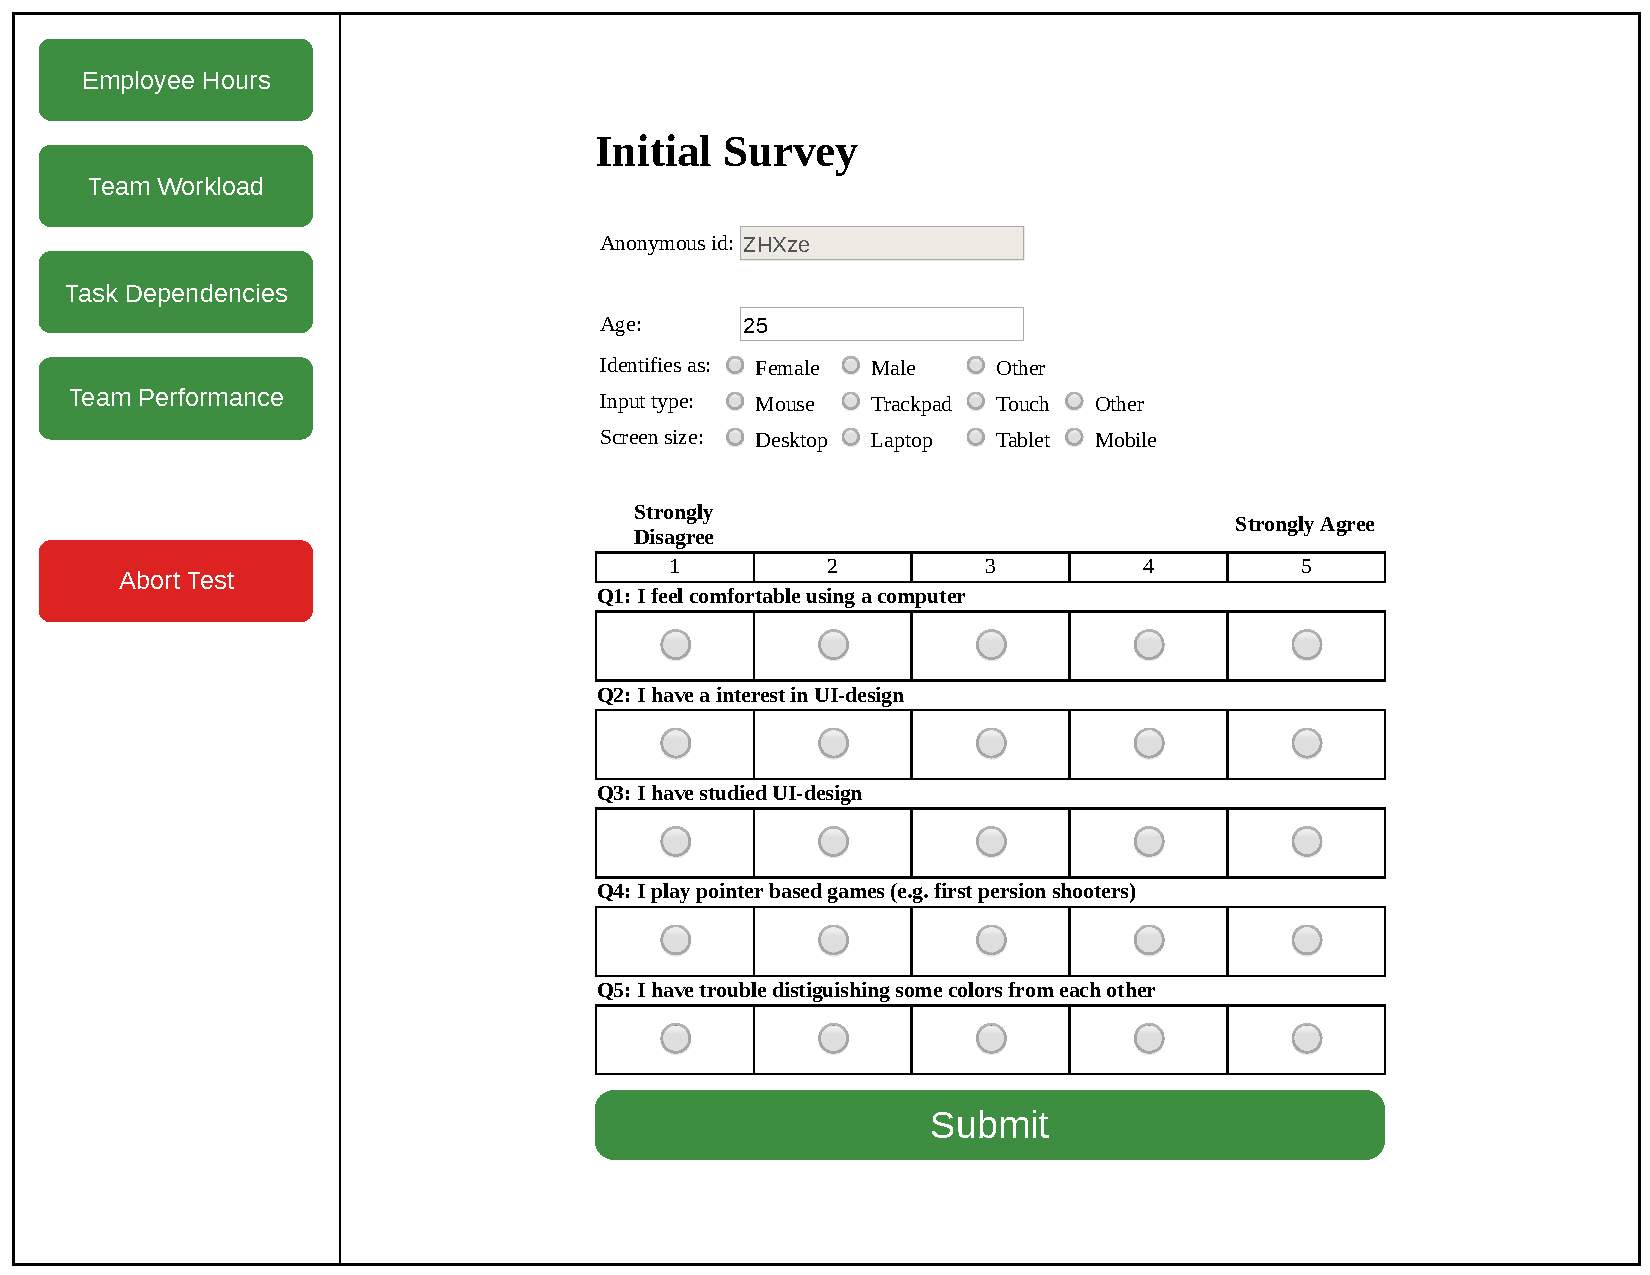
\includegraphics[width=.7\textwidth]{figures/captures/webapp_pre_survey.pdf}
          \caption{Capture of initial survey page.}
          \label{label_preSurvey}
        \end{figure}

        While it is possible for the participant to interact with the buttons on
        the left side before the initial survey is submitted, pressing any of the
        buttons except 'Abort Test' will only display the same survey-page.

        \begin{figure}[h!]
          \centering
          \fbox{
            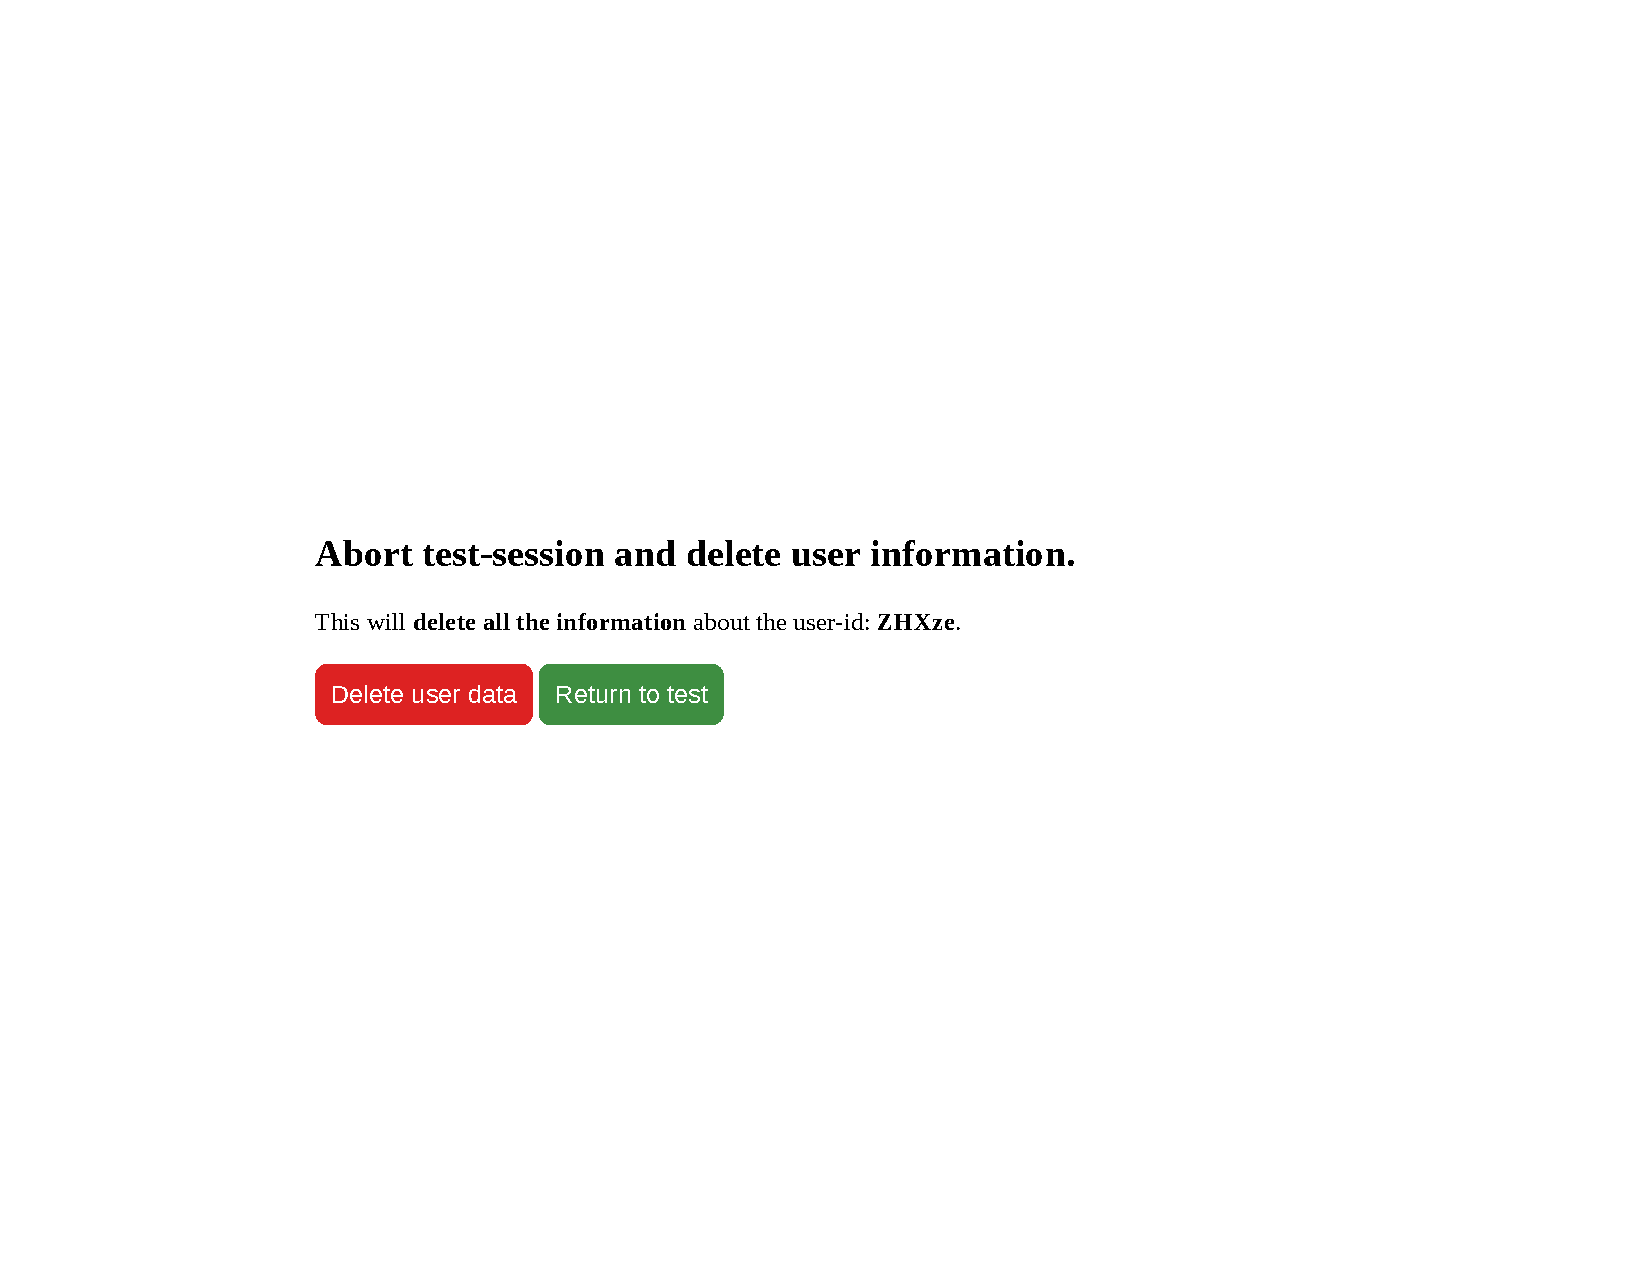
\includegraphics[trim={4cm 8cm 9cm 8cm},clip,width=.5\textwidth]{figures/captures/webapp_abort.pdf}
          }
          \caption{Capture of confirmation page for aborting the test.}
          \label{label_abort}
        \end{figure}

        The dedicated 'Abort Test' button is available in all the different
        views of the application, in case the participant no longer wants to
        participate for any reason. Pressing this button displays a page
        explaining that continuing will scrub any activity related to their
        current anonymous id from the database and abort the current test.
        %Additionally and return it to the pool
        %of available identification strings.


      \subsection{Landing page}

        After the participant has submitted the pre-survey, it  disappears and is
        replaced by a few basic statistics about the current test session.
        The functionality of the left-side buttons is restored and makes it
        possible to choose any of the following four test types:
        \textit{Employee Hours},
        \textit{Team Workload},
        \textit{Task Dependencies} and
        \textit{Team Performance}.

        \begin{figure}[h!]
          \centering
          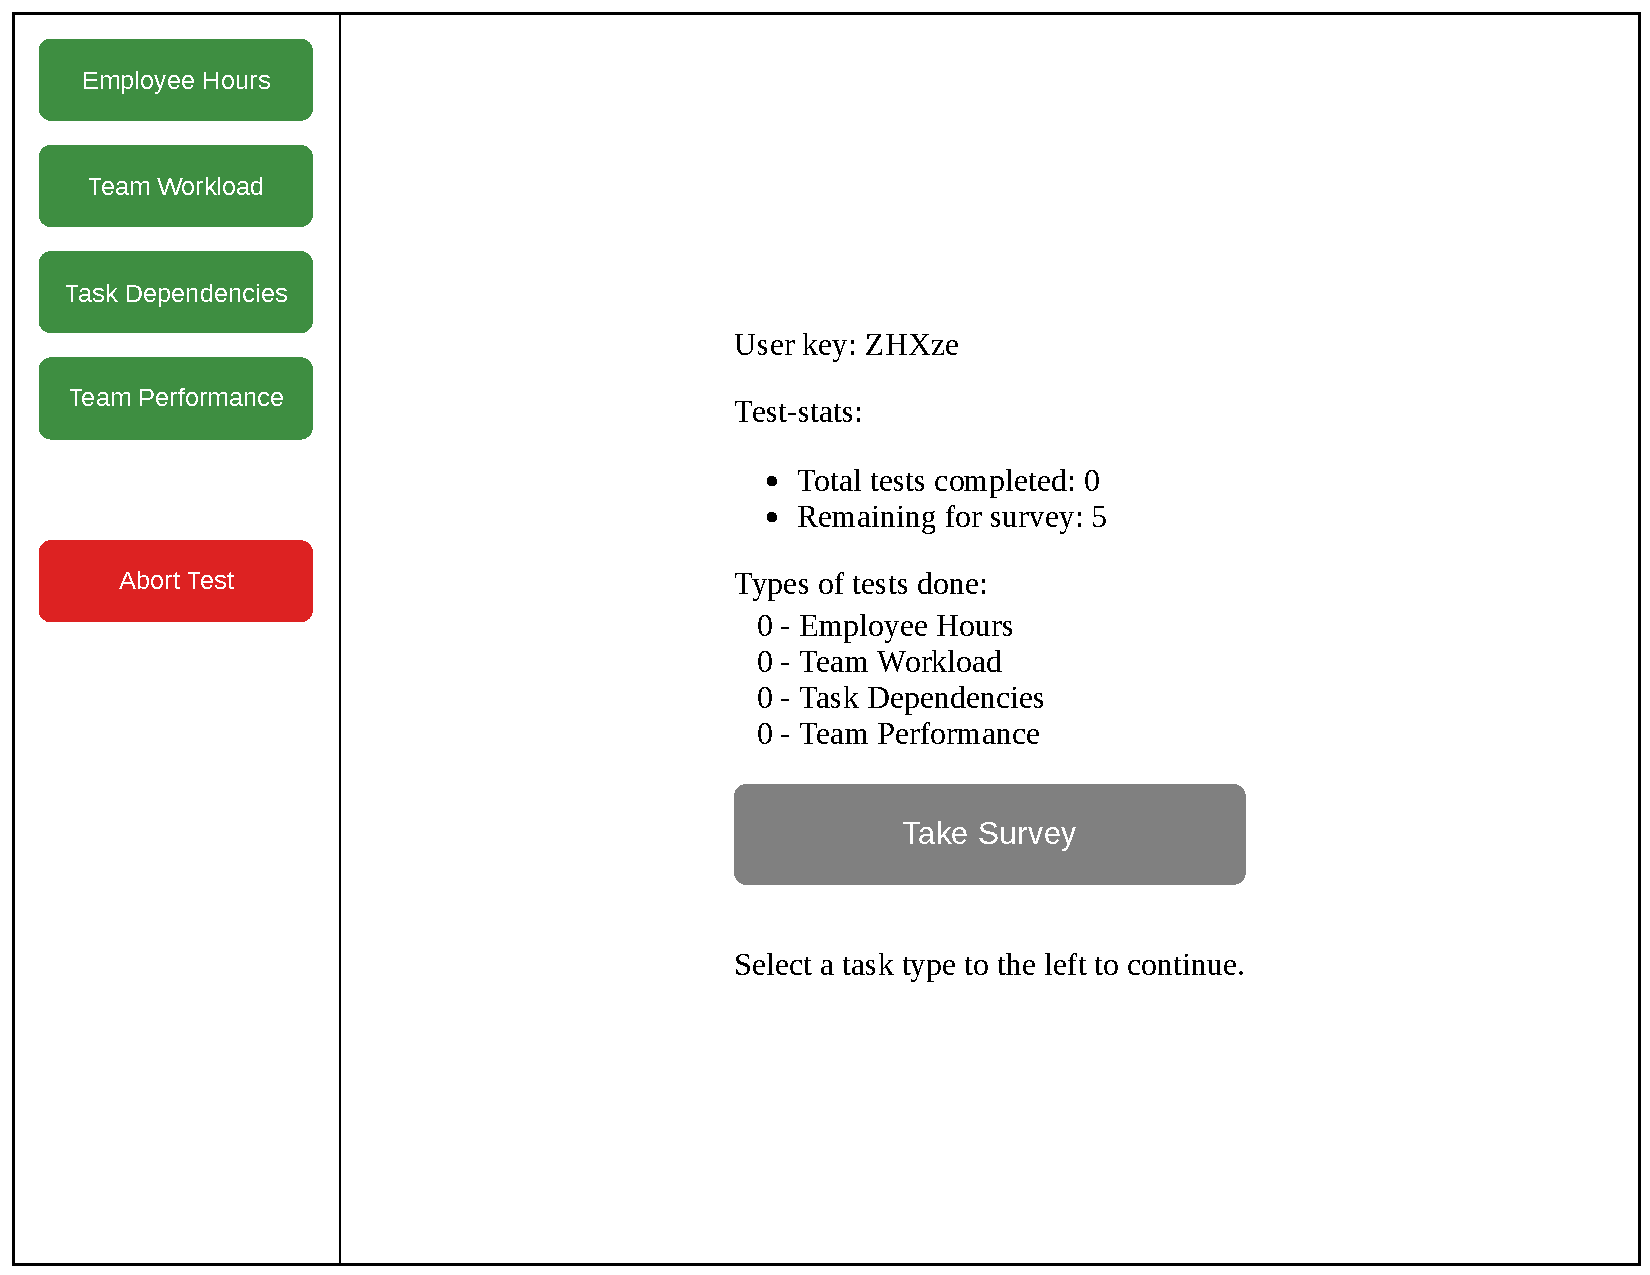
\includegraphics[width=.7\textwidth]{figures/captures/webapp_main_statistics.pdf}
          \caption{Capture of the hub page, post initial survey, default state.}
          \label{label_mainStatistics}
        \end{figure}

        The session-statistics include the participants assigned anonymous id,
        how many test of each type they have completed and how many test they
        have to complete in order for the post-survey to become available.

        Requiring five tests before making the post-survey available is the only
        hard limitation placed on the participants. Other than the test-minimum
        there is no limit on how many tests they can perform or how long time
        they take to complete a individual test or the test session as a whole.

      \subsection{Information, fictional context and execution}

        Before starting any of the tasks, the participant is greeted by a page
        containing the general information about the task at hand. Each of the
        pages follows the same structure with three sections, \textit{Goal},
        \textit{How} and \textit{Summary}, explained below.
        \todo{Re-edit}

        The \textit{Goal} section should be short{\findref}, a sentence at
        most{\findref}, and tell the participant what they need to do in order
        to complete the task successfully.

        After reading the \textit{How} section, the participant should have a
        basic understanding of how the information related to the test is
        structured and presented. If there are any specific details about the
        representation of the task that are deemed essential they should be
        described in this section.

        The \textit{Summary} section is meant to repeat the information in the
        \textit{How} section, but in a different and briefer fashion in order
        to help with retention\findref.

        Lastly, the participant is told that the same information that has just
        been presented is available after starting the test, accessible by
        hovering the cursor over a '?' in the upper left corner.

        Since all the task-mechanics boil down to
        \textit{find the element and press it as fast as possible},
        the intent is to give the participant enough concrete
        information about the test at hand while trying to maintain the
        implied fictional context of the task. Which means the tone of any
        instructions or information should be closer to
        \textit{''select the co-worker with the most X''} rather than
        \textit{''click the largest box''}.
        \todoMaybe{Colorswatches}
        \todoMaybe{Range of values}
        \todoMaybe{Randomization-1 + max}
        \todoMaybe{Add about no feedback on result -> BAD}

      %pallet = [
      %  "#001f3f",
      %  "#0074D9",
      %  "#39CCCC",
      %  "#3D9970",
      %  "#2ECC40",
      %  "#01FF70",
      %  "#FFDC00",
      %  "#FF851B",
      %  "#85144b",
      %  "#F012BE",
      %  "#B10DC9"
      %]

%      \subsection{Task - employee hours}
      \subsection{Employee hours}

        \textit{\ideaOne}

        The premise for this task is that the organization generating the data
        utilizes some form of task assigning system together with a
        cost-estimation system. In short, there is a set of tasks that need to
        be done, each with a estimated time-cost, and a number of people that
        can be scheduled to do said work.

        Given there is a limited amount of time that any assignee can spend
        working, it is possible to over-schedule someone. In this scenario,
        being over-scheduled is the result of having more work scheduled to you
        over a period of time than the total available capacity for the same
        period. In summary, the goal of this task consists of identifying these
        cases, in particular, the person that is the most over-scheduled.

        \begin{figure}[h!]
          \centering
          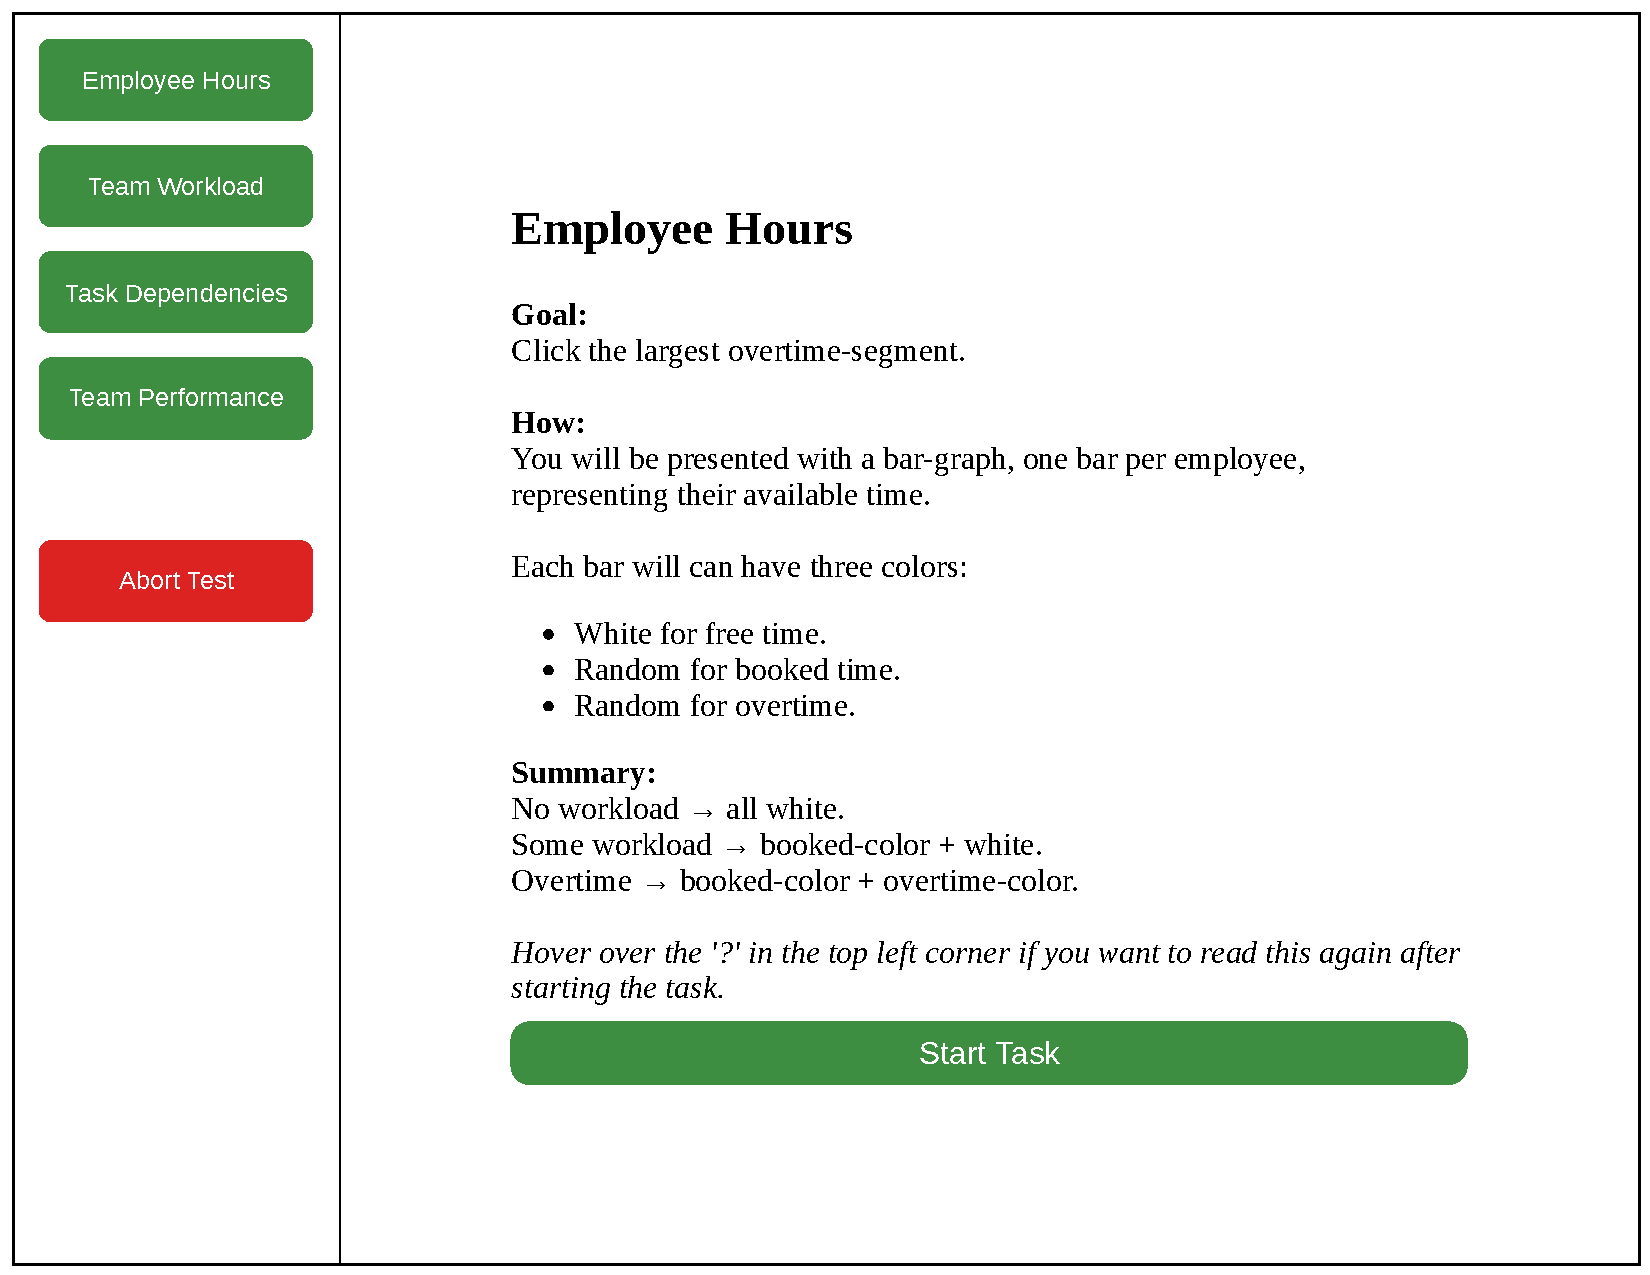
\includegraphics[width=.49\textwidth]{figures/captures/webapp_employee_hours_info.pdf}
          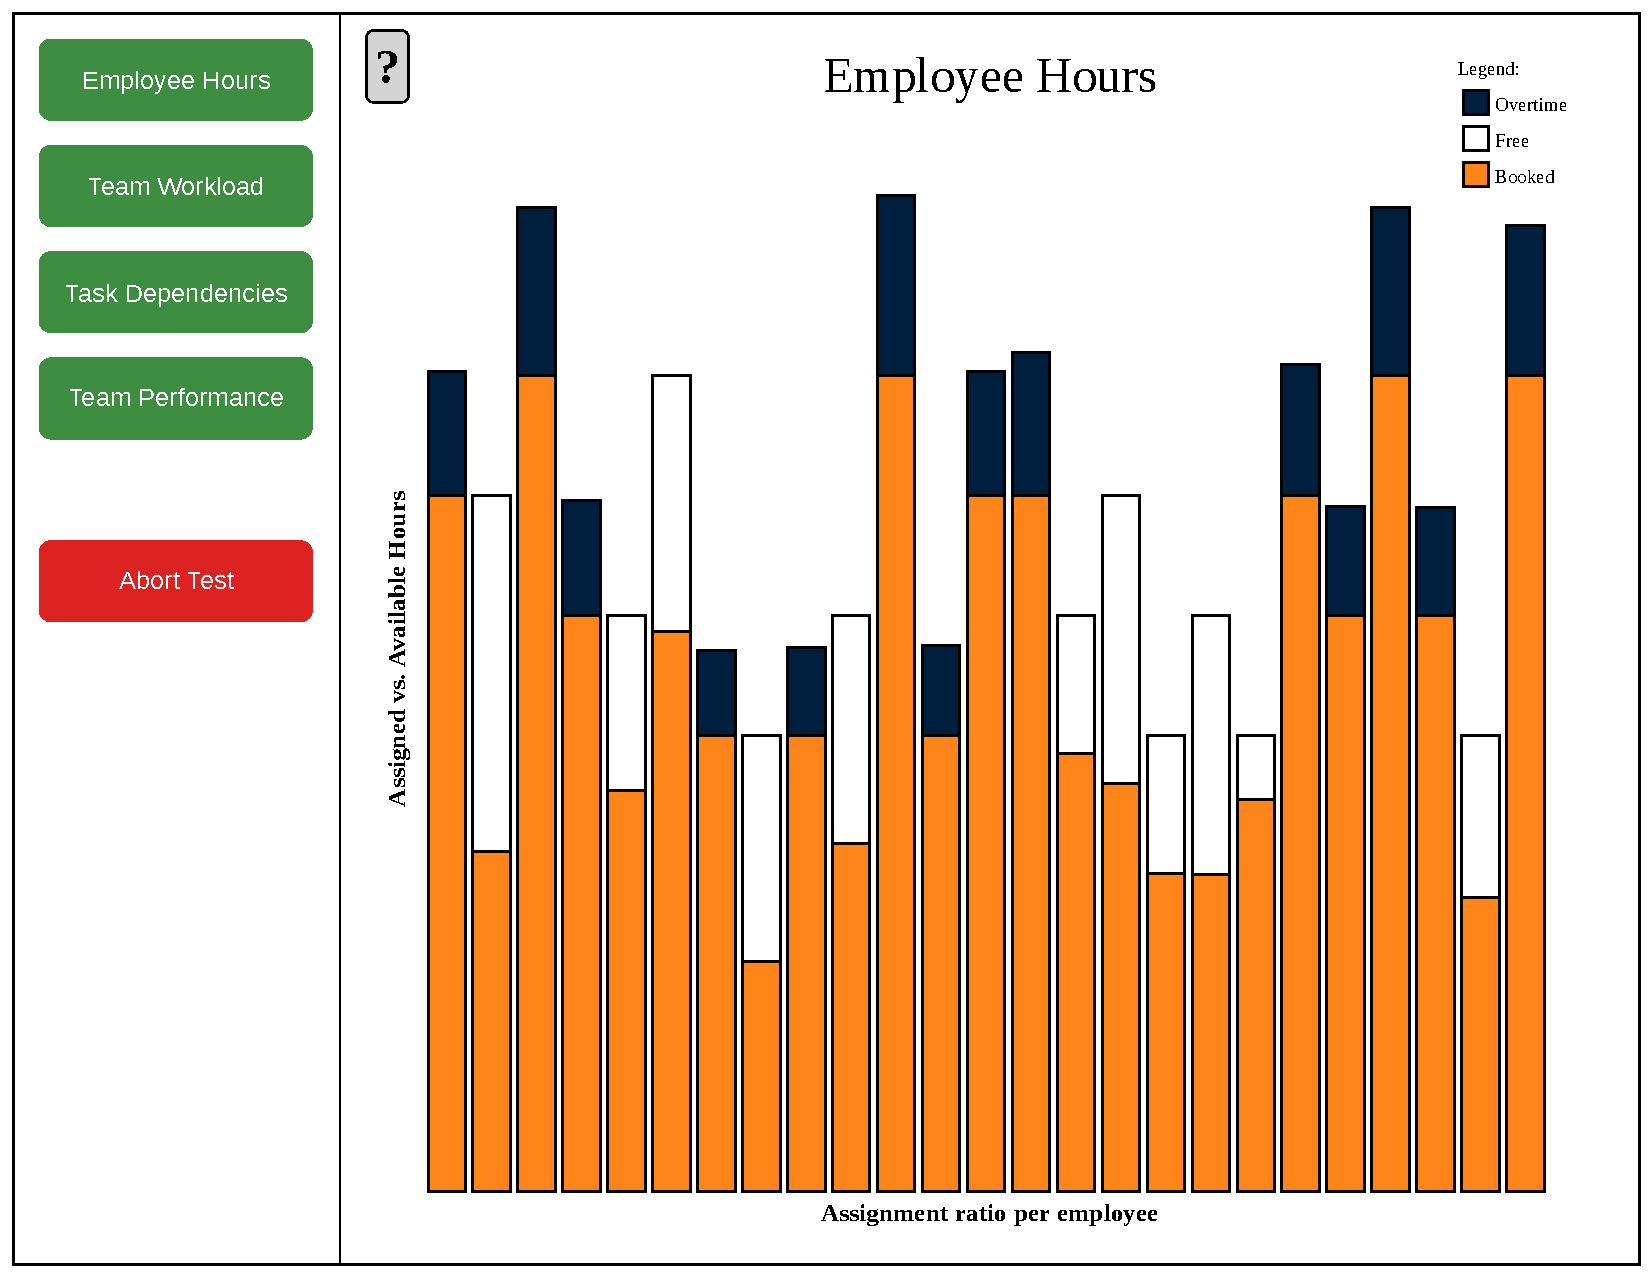
\includegraphics[width=.49\textwidth]{figures/captures/webapp_employee_hours_task.pdf}
          \caption{Capture of Employee Hours information and task page.}
        \end{figure}

        After starting the task, the participant is shown a bar-graph with bars
        of varying heights and coloring. Each bar shows the relation between
        available and scheduled work-time for one out of the twenty-five
        represented people.

        Here, the height of the black outline of each bar represents the
        \textit{available work-capacity}, the varying heights simulating the
        difference of available hours due to to sick-leave, vacations or
        different contracts.

        The \textit{total scheduled workload} for
        each person is represented by the height of the colored segments in
        each bar. If there is capacity left the colored segment will not extend to the
        top of the bar outline, leaving a white segment representing
        non-scheduled time. On the other hand, if the amount of scheduled work
        is greater than the available capacity, the color will extend beyond
        the original outline and be colored differently for readability.

        In summary, the height of a white segments in a bar represent the
        amount of remaining capacity, while the height of any other-colored
        segment signifies how \textit{over-scheduled} someone is. Find the
        largest other-colored segment it and click on it.

%      \subsection{Task - team workload}
      \subsection{Team workload}

        \textit{\ideaTwo}

        In the following scenario the business or organization has a schedule,
        Monday to Friday, that stretches twenty-five weeks into the future. The
        goal is to keep the workload as steady as possible without to many
        jumps in either direction. Have to little to do and people are
        underutilized and in worst case, bored. Have to much that needs to be
        done at the same time and people might burn out. Avoiding both
        extremes would be preferable.

        \begin{figure}[h!]
          \centering
          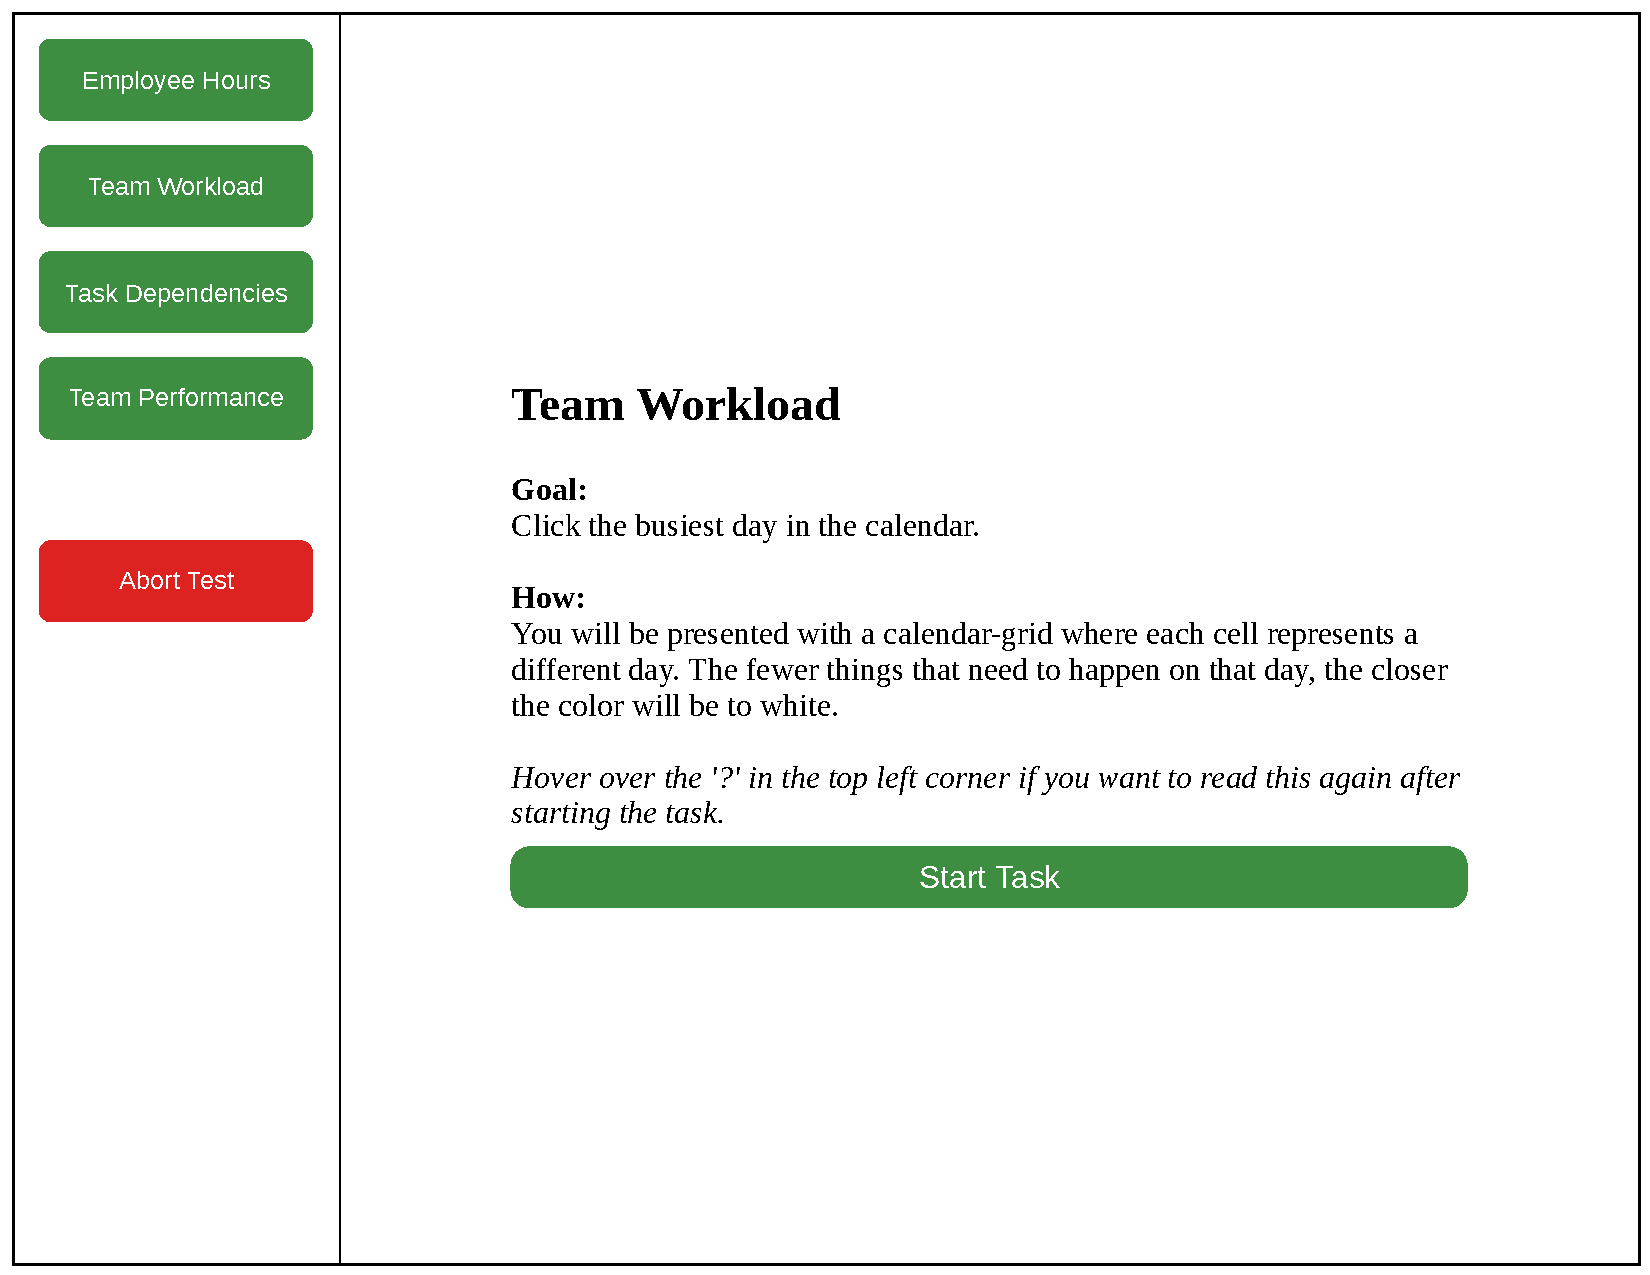
\includegraphics[width=.49\textwidth]{figures/captures/webapp_team_workload_info.pdf}
          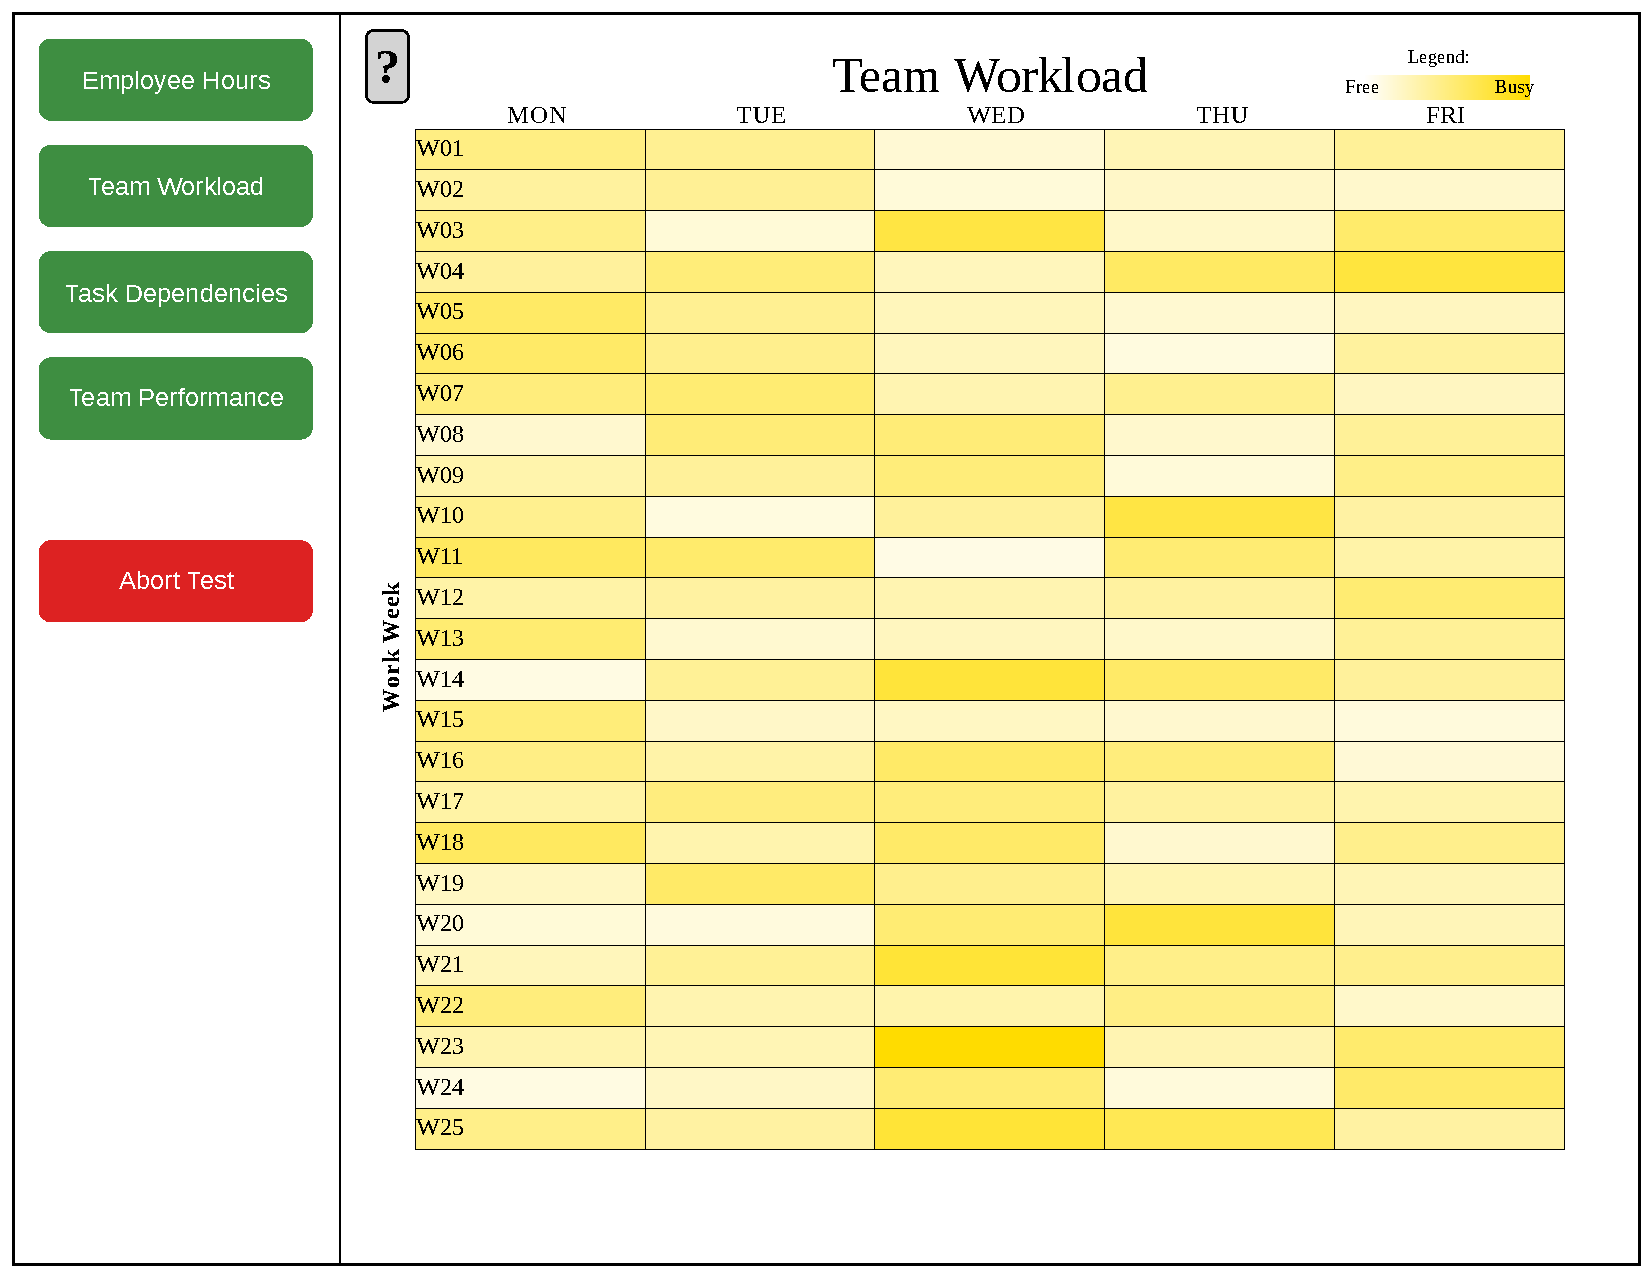
\includegraphics[width=.49\textwidth]{figures/captures/webapp_team_workload_task.pdf}
          \caption{Capture of Team Workload information and task page.}
        \end{figure}

        Running this test shows the participant a grid of twenty-five rows
        consisting of five columns each, denoted
        \texttt{MON},
        \texttt{TUE},
        \texttt{WED},
        \texttt{THU} and
        \texttt{FRI},
        representing the scheduled twenty-five workweeks mentioned above. Each
        of the rectangles are colored with the same color but differ in the
        saturation. A cell that has zero saturation, or white in this case,
        signal that no work is scheduled for completion on that particular day.
        Inversely, the darker a cell is, the more work needs to be completed on
        that specific day.

        Since there needs to be a clearly defined goal for each test, there has
        to be a choice between bored and burned out people, where the latter
        seems far worse. Now the problem can be corrected by identifying days
        where there is an extra high amount of work that needs to be done, and
        try to re-schedule it to less busy days.

        For the participant executing the test, the goal is to find the
        darkest, or most saturated rectangle and click it as fast as possible.

      \subsection{Task dependencies}

        \textit{\ideaThree}

        The assumption for this test is that the underlying system producing
        the data has tasks that need to be completed first in order for other
        tasks to complete in turn, in short, dependencies. This test revolves
        around answering the question
        \textit{''which elements are the most crucial for the overall
          process?''}. The answer to this question can be very useful, as an
        example, when being forced to cut back on things due to limited
        resources while trying to affect as few other things as possible.

        \begin{figure}[h!]
          \centering
          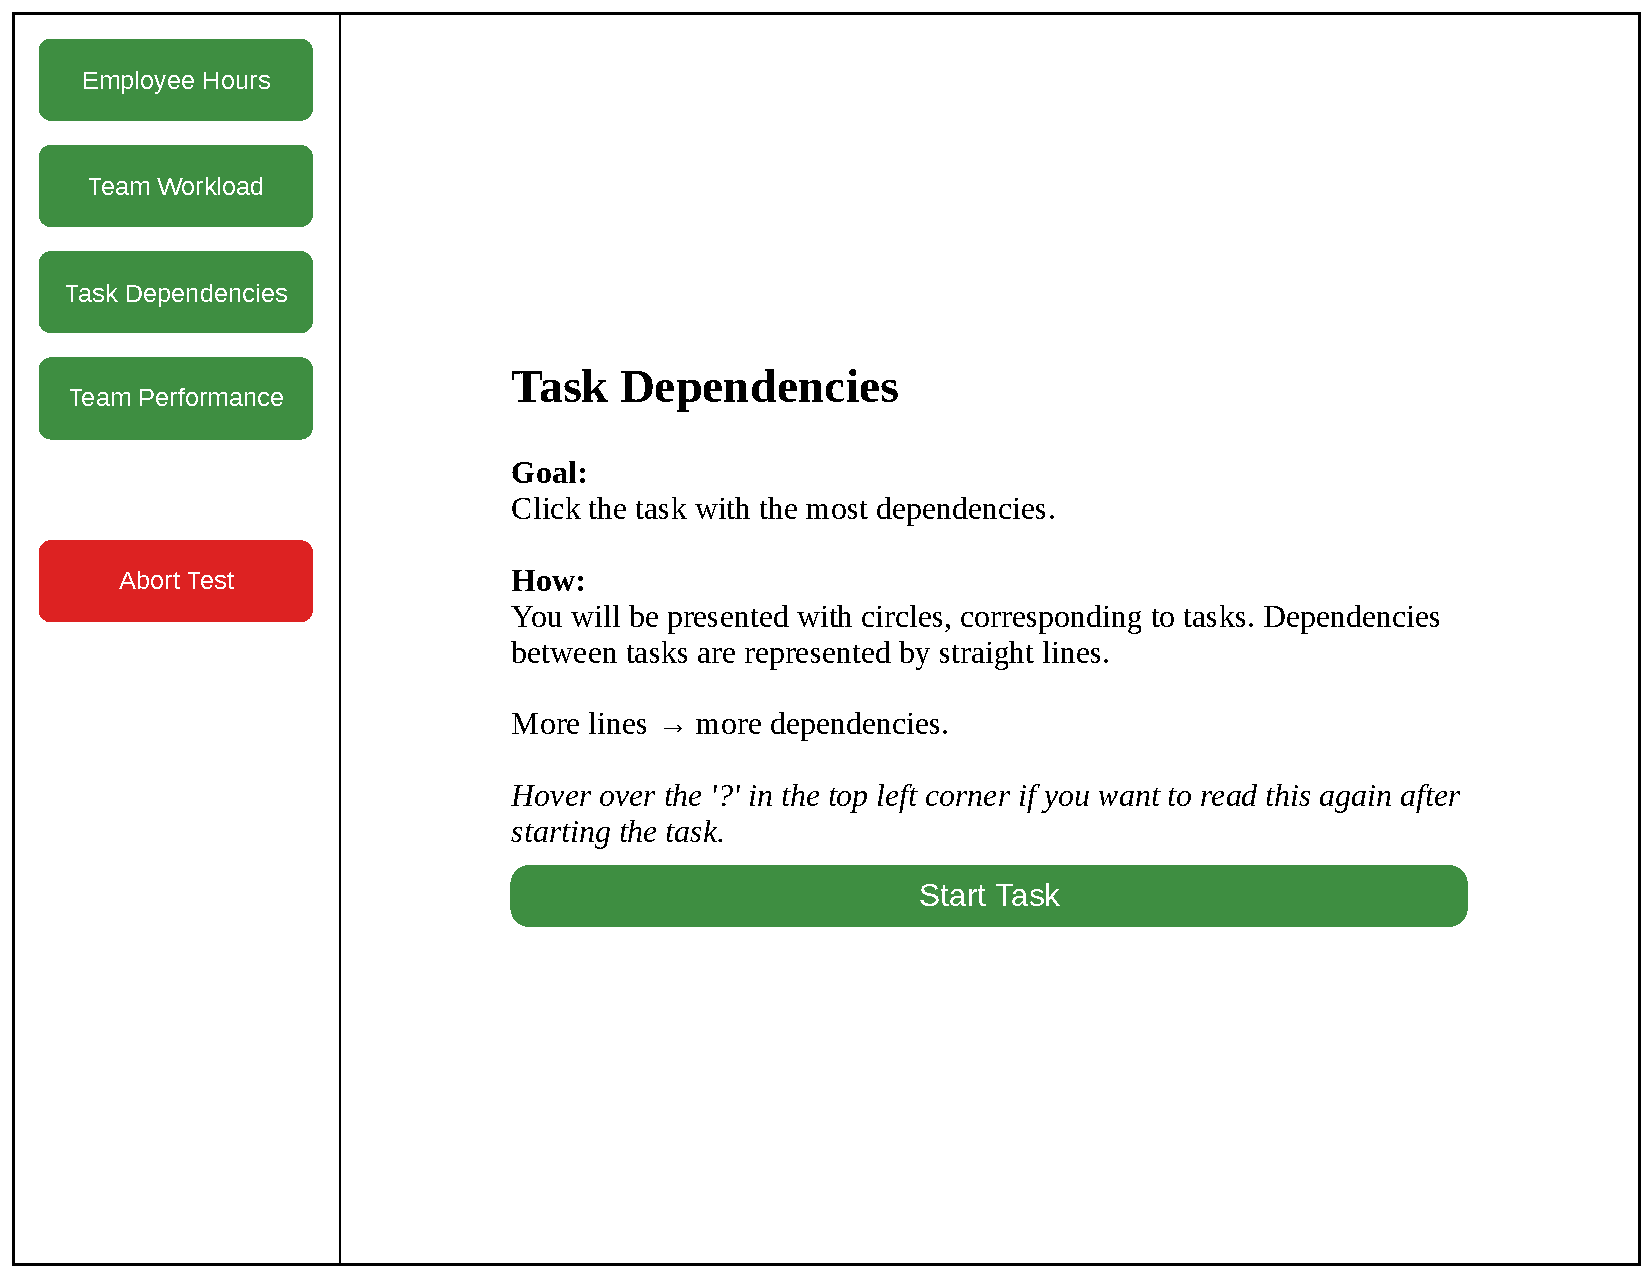
\includegraphics[width=.49\textwidth]{figures/captures/webapp_dependencies_info.pdf}
          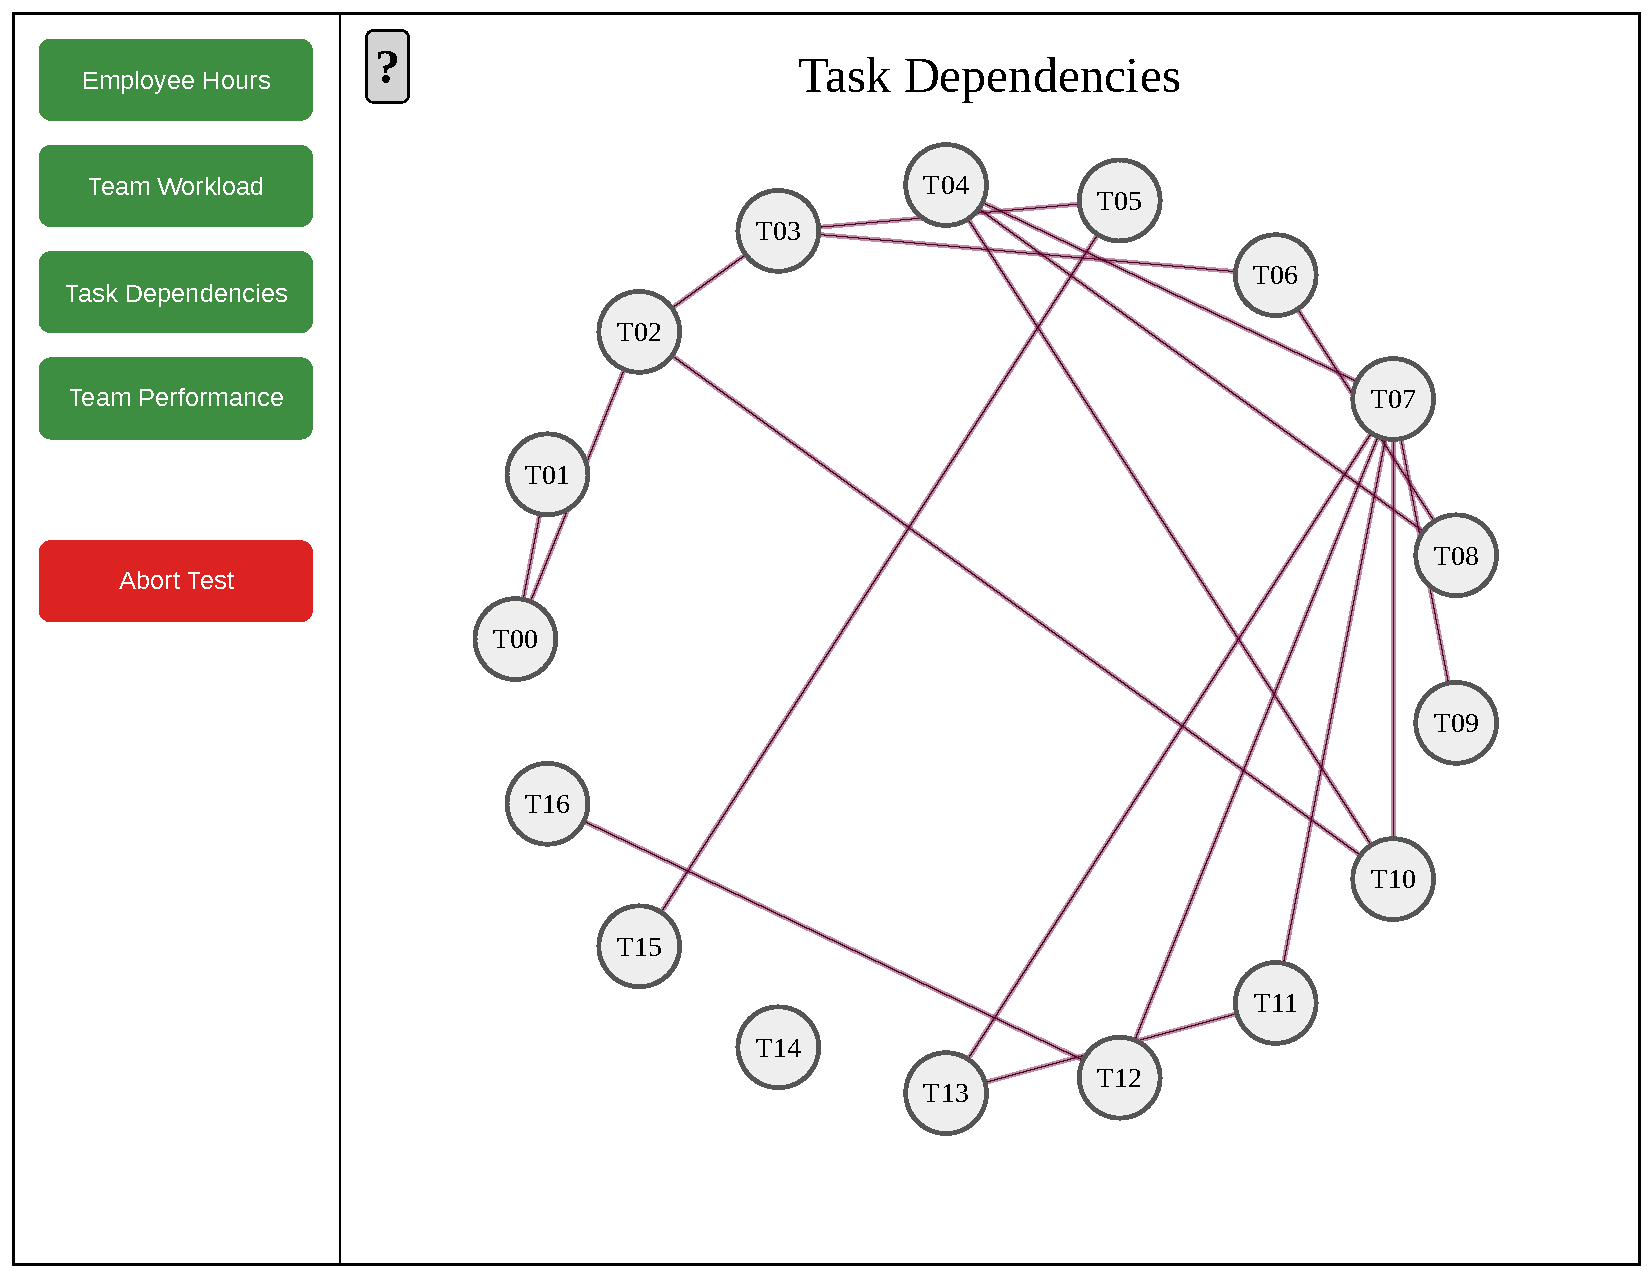
\includegraphics[width=.49\textwidth]{figures/captures/webapp_dependencies_task.pdf}
          \caption{Capture of Task Dependencies info- and task-page.}
        \end{figure}

        Initializing this test shows the participant seventeen small circles,
        representing tasks, arranged in a larger circle. Additionally, there are
        colored lines connecting some circles together, indicating there is
        a dependency between them, more lines equals more dependencies.

        Since the stated interest in knowing how dependent the different
        moving parts are on each other, knowing which task has the most
        dependencies is a good start. In terms of what the participant has to
        do to finish the test, this translates to; find the task with the most
        connections and click on it as fast as possible.

       % \subsection{Task - team performance}
        \subsection{Team performance}

        \textit{\ideaFour}

        Given a working-environment where things are done in parallell it
        becomes interesting to know if a specific group or individual is
        especially effective in a certain area. Having this information makes
        it possible to assign people, if they excel at a specific area, to
        tasks that match their abilities.

        In this test there are five different task-categories,
        \textit{tickets},
        \textit{rnd},
        \textit{support},
        \textit{features} and
        \textit{maintentance}.

        \begin{figure}[h!]
          \centering
          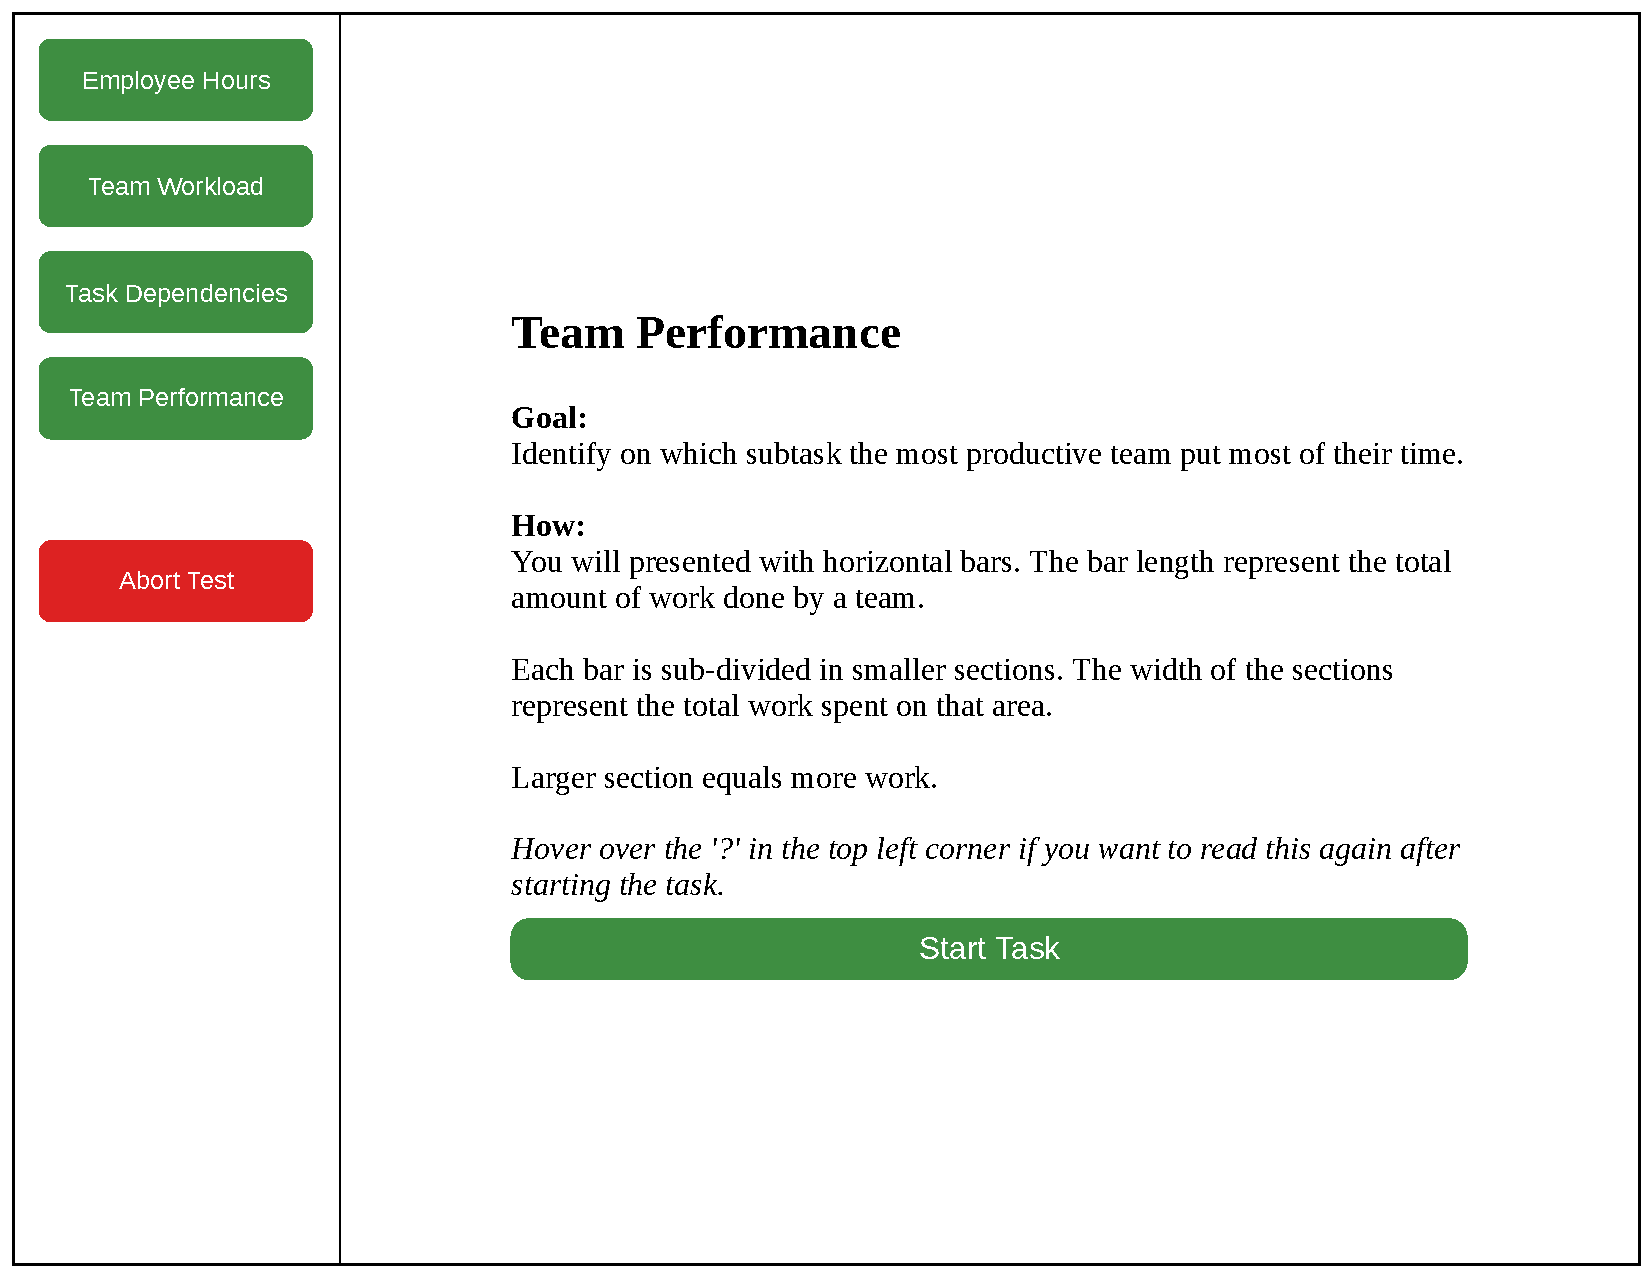
\includegraphics[width=.49\textwidth]{figures/captures/webapp_team_performance_info.pdf}
          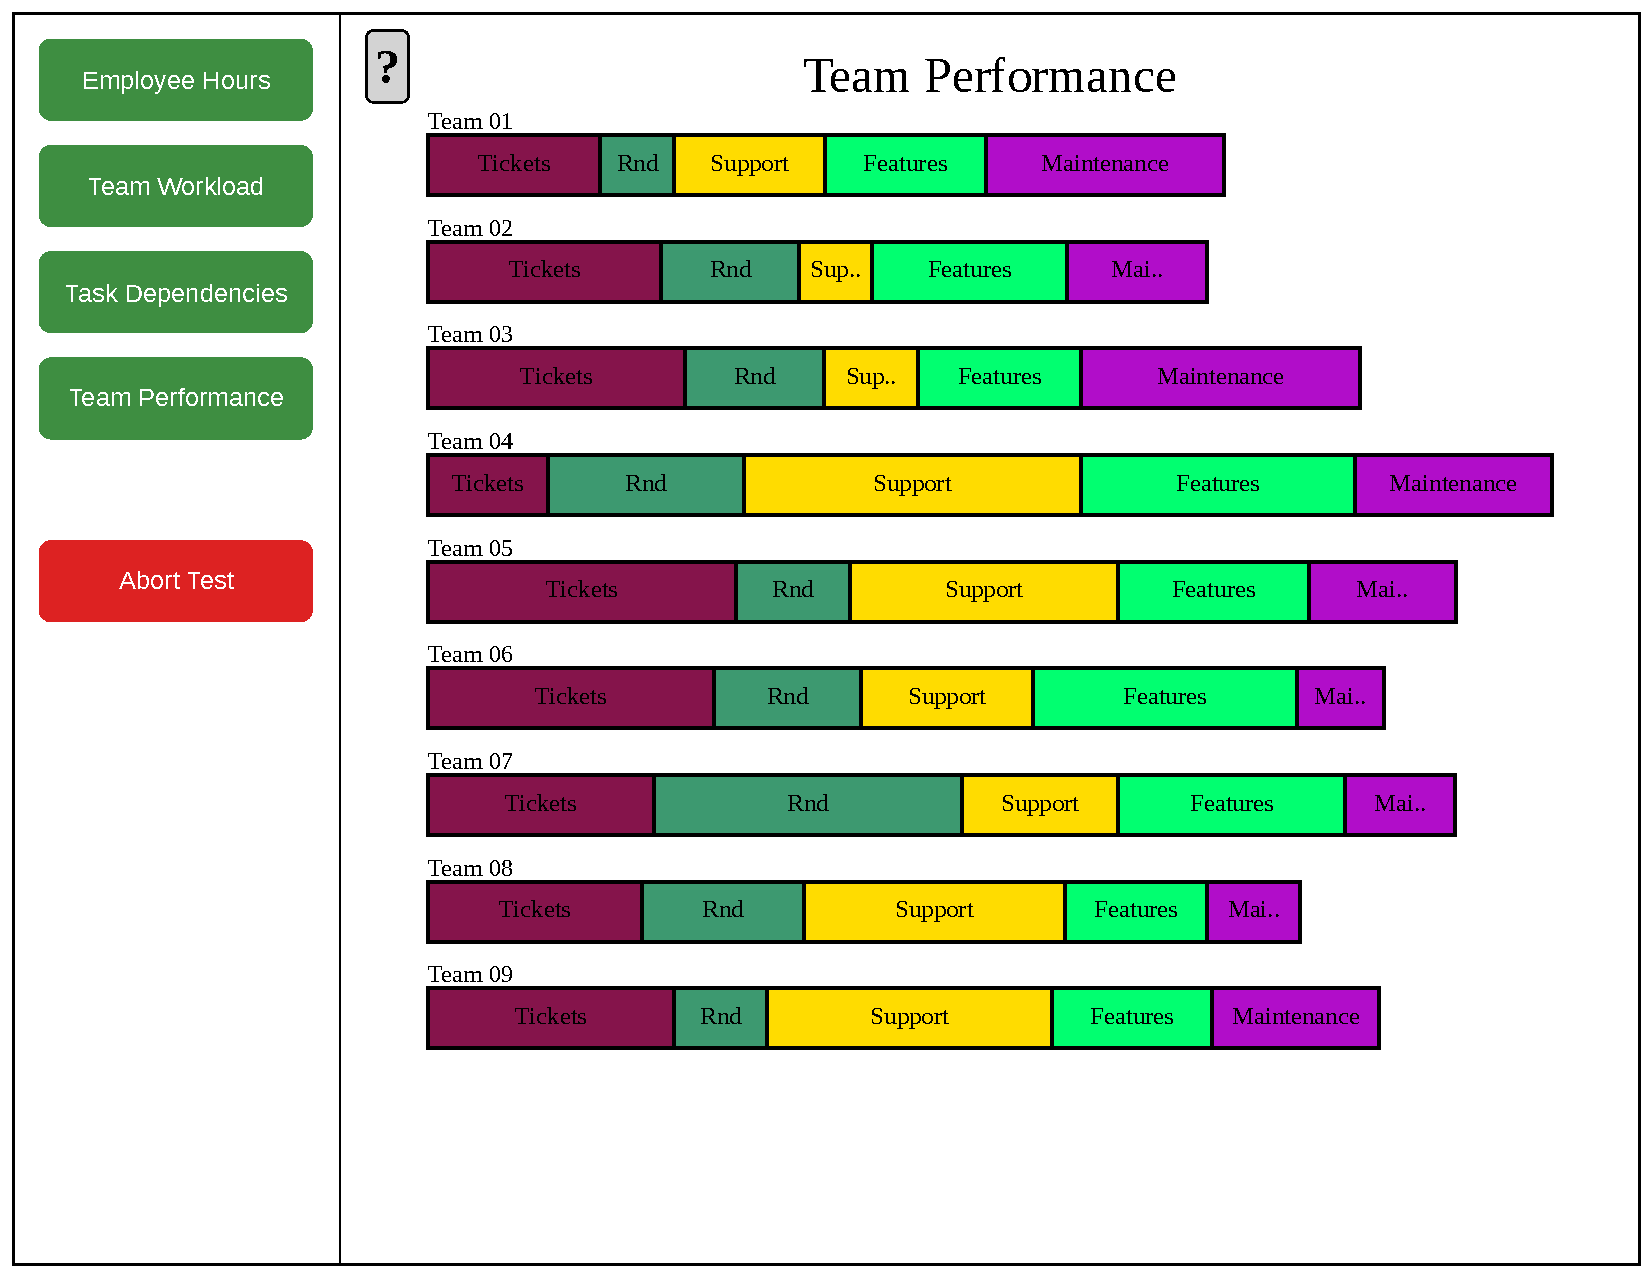
\includegraphics[width=.49\textwidth]{figures/captures/webapp_team_performance_task.pdf}
          \caption{Capture of Team Performance info- and task-page.}
        \end{figure}

        This task presents the participant with bars showcasing the total
        completed work-load for nine different teams over an unspecified amount
        of time.

        There are two types of information shown, the total amount of work done
        by each team, represented by the total horizontal length of the bar.
        And the amount of the total work that went into a specific
        task-section, represented by the length of each individual sub-section
        of the overall bar.
        In order to correctly answer this test, the participant first needs to
        identify which of the bars is the longest one, and then identify which
        sub-section is the largest one, and click on that one.

      \subsection{Post survey}

        As the participant completes five or more tests the 'Take Survey'
        button becomes active, pressing this button sends the participant to
        the post-survey page. Other than the survey itself, there is also the
        option to return to the tests if the button was pressed by accident or
        if the participant had a change of mind.

        The post-survey consist of eight questions and an optional input field
        for additional comments. These questions are ment to evaluate the
        participants thoughts about the current iteration of the testing
        application in order to derive possible improvement for the next
        implementation iteration.

        Options that are of interest include, among others, if the goal of each
        task was clear, if the application was pleasing to look at, if the use of
        colors help when navigating application, etcetera. For a verbatim list of
        the questions used in the post-questionnaire see figure
        \todoInsert{reference to post-survey}.

		\section{Results}

			\subsection{Pre-questionnaire -- itemizations}

        Before being able to perform the test, each participant has to fill
        out and submit a pre-questionnaire. This is done in order to get
        a rough demographical overview of the people participating in this
        study. Initially they are asked about age, used input device, type of
        screen category the test were conducted on, and what binary gender, if
        any, they identify as.

				\begin{figure}[h!]
					\centering
					\includegraphics{figures/preQuestionnaireAnswers.pdf}
					\caption{Answers for the pre-questionnaire.}
				\end{figure}

        Beginning with age, with each dot representing one answer, no
        participant was twenty or below, most of the  participants were between
        twenty-one and thirty-five, with fourteen being thirty-six and older.
        Since a large part of the participants came from MASSIVE, this seems to
        fit the mean age at the company, which is at thirty-two{\findref} at
        the time of this writing.

        It's is worth mentioning however, that the most represented single age
        was twenty-five, which is the default value set for the age input
        field. More on this specifically in \todoInsert{Link to threats to
          validity}.

				\begin{figure}[h!]
					\centering
					\includegraphics{figures/preQuestionnaireAnswersIdentify.pdf}
					\caption{Answers for the pre-questionnaire.}
				\end{figure}

        Asking people for what gender they identify as results in the largest
        group, 52 participants, identify as male. Again, as a large portion of
        participants came from MASSIVE, this is expected since the gender
        distribution in businesses related game-development tend to be weighted
        toward men\findref\findref.

				\begin{figure}[h!]
					\centering
					\includegraphics{figures/preQuestionnaireAnswersInputs.pdf}
					\caption{Answers for the pre-questionnaire.}
				\end{figure}

        Continuing the trend, most workstations at MASSIVE consist of a
        desktop PC where the main peripherals used for input are a mouse and a
        keyboard with the occasional drawing tablet mixed in.

        In general it was assumed that most of the participants were going to
        use a mouse and keyboard, with trackpads as a probable second place,
        making the turnout of nearly twenty participants using touch as their
        main input a bit of a surprise.

        Even though the assumed main input method for these tests is a keyboard
        and mouse at a stationary desktop computer, the overarching goal of the
        project, as stated earlier, is to be a pre-cursor to o more generalized
        usability testing framework. In order to align with this goal, it is
        important to explore the possibility of scaling the interface and
        related tests to different screen sizes, and analyze what, if any,
        impact is has on participant performance.

				\begin{figure}[h!]
					\centering
					\includegraphics{figures/preQuestionnaireAnswersScreen.pdf}
					\caption{Answers for the pre-questionnaire.}
				\end{figure}

        Requiring actual screen-sizes was seen as to cumbersome of a task to
        ask of the participants, especially if using devices other than a
        somewhat standard desktop monitor. Here the categories roughly equate
        to; \textit{Desktop}: 18" or larger, \textit{Laptop}: 13"-17", \textit{Tablet}:
        11"-12" and \textit{Mobile}: 10" and below.

			\subsection{Pre-questionnaire -- 1-5 questions}

        Aside from the physical setup, there are relevant knowledges and
        experience that could become interesting when analyzing free-form
        answers and test-results gathered from the participants. As an example,
        is the free-form feedback different from someone that is interested in
        usability-design? Does the level of computer literacy or experience
        with mouse-driven games impact completion times? Etcetera.

        In order to evaluate these aspects the second half of the
        pre-questionnaire included five self-evaluation-1-to-5 questions
        \todo{Find the actual name}, questions and answer distribution
        displayed below:

				\begin{figure}[h!]
          \textbf{Q1: I feel comfortable using a computer.}
          \begin{center}
            \includegraphics[width=\linewidth]{figures/preQuestionnaireAnswersOneToFive.pdf}
            \vspace{-1cm}
            \caption{Answers for the pre-questionnaire Q1.}
          \end{center}
				\end{figure}

        The clear majority of participants feel that they are very comfortable
        using a computer. Since this question is so heavily skewed towards
        \textit{Strongly agree}, it would be interesting to add an additional
        \textit{I see myself as an advanced computer user} or similar in order
        to try to separate out more divisions.

				\begin{figure}[h!]
          \textbf{Q2: I have a interest in UI-design.}
          \begin{center}
            \includegraphics[width=\linewidth]{figures/preQuestionnaireAnswersOneToFiveQ2.pdf}
            \vspace{-1cm}
            \caption{Answers for the pre-questionnaire Q2.}
          \end{center}
				\end{figure}

        Looking at the general interest in regards to user interface design,
        most participants either do not care about it, or find it somewhat to
        very interesting. If this was a non-anonymous study, it would be
        interesting to follow up on the seven participants that strongly
        disagree to this question. Mostly in order to differentiate if they do
        not like user interfaces an input method in general, or if it is more
        related to them not wanting to be involved in user interface design.

				\begin{figure}[h!]
          \textbf{Q3: I have studied UI-design.}
          \begin{center}
            \includegraphics[width=\linewidth]{figures/preQuestionnaireAnswersOneToFiveQ3.pdf}
            \vspace{-1cm}
            \caption{Answers for the pre-questionnaire Q3.}
          \end{center}
				\end{figure}

        In terms of having studied user interface design, the majority of
        participants have not. Since this is a pure self-assessment, the
        definition of what \textit{studied} means in this context is up for
        grabs. A follow up question in regards to what type of study;
        self-learnt, online-course, university etcetera would be needed clarify
        this information further.

				\begin{figure}[h!]
          \textbf{Q4: I play pointer based games (e.g. first person shooters).}
          \begin{center}
            \includegraphics[width=\linewidth]{figures/preQuestionnaireAnswersOneToFiveQ4.pdf}
            \vspace{-1cm}
            \caption{Answers for the pre-questionnaire Q4.}
          \end{center}
				\end{figure}

        A slight majority agree, in some capacity, that they play games where
        the main form of input is pointer movements. Following this question
        with one that seeks to answer the underlying reason why disagreeing
        participants do not interact more with this kind of games could be
        interesting from a interface design standpoint. Additional questions or
        follow-up would be needed to determine if the disagreement it is a
        matter of taste, design faults, available time, or something completely
        different.

				\begin{figure}[h!]
          \textbf{Q5: I have trouble distinguishing some colors from each other.}
          \begin{center}
            \includegraphics[width=\linewidth]{figures/preQuestionnaireAnswersOneToFiveQ5.pdf}
            \vspace{-1cm}
            \caption{Answers for the pre-questionnaire Q5.}
            \vspace{-0.4cm}
          \end{center}
				\end{figure}

        All of the available tests incorporates different color pallets to
        varying degree, which makes it interesting to know if any of the
        participants have trouble making out the difference between colors.
        \vspace{-0.6cm}

			\subsection{Launch, participation and overall success ratio}

        The test-site went live 2020-01-24 with the link initially shared only
        through Facebook. On 2020-01-27 the link was shared on the MASSIVE
        internal mailing list, boosting the participation significantly.
        In total, \varHere{totalParticipants} participants moved past the
        initial information over a five day period.

				\begin{figure}[h!]
					\centering
					\includegraphics{figures/participantsOverTime.pdf}
          \vspace{-0.3cm}
          \caption{
            Total amount of participants that got past each of the milestones
            defined in figure \ref{label_milestones}.
          }
				\end{figure}

				In total \varHere{totalTests} tests were run, where
				\varHere{totalTestsCorrect} were answered correctly,
				\varHere{totalTestsUncompleted} never produced an answer, leaving
				\varHere{totalTestsIncorrect} incorrect answers. Looking only on the test
				runs without any user- or task-correlation, the chance that any given test run
				produces the correct answer is $\sim$\varHere{varTotalRatioSuccess}\%.

				\begin{figure}[h!]
					\centering
					\includegraphics[width=0.95\linewidth]{figures/runsOverTime.pdf}
          \vspace{-0.3cm}
          \caption{Lines representing total amount of test-runs together with
            the total of runs that produces the correct answer.}
          \vspace{-0.4cm}
				\end{figure}

			\subsection{Tests per user and defining outliers}

				The number of recommended test was five, which when completed, allowed
				the participant to continue to the final survey. However, there was
				nothing stopping each participant from doing more or less than five.
        By generating a histogram for the number of performed tests per
        participant it is possible to determine which of tests was most
        popular.

				\begin{figure}[h!]
					\centering
					\includegraphics{figures/testsPerUser.pdf}
					\caption{Participants grouped on how many test they performed.}
				\end{figure}

        In total, of the \varHere{totalParticipants} number of participant that
        started a session, \varHere{valNumAnyTestsRun} of them ran at least one
        test, which means \varHere{valTestNoTests} ran no tests. Retrieving and
        tabulating additional values, discarding users with no test-runs,
        produces the following table.

        \begin{figure}[h!]
          \centering
          \varHere{tablePrecentageOfUsers}
          \caption{%
            Tabulated values of test-run groups with corresponding percentage
            of total active participants.%
          }
        \end{figure}

        Participants that have run at most fifteen tests make up slightly more
        than 91\% of the total number of participants and will be the regular
        group, denoted as $\#r\leq15$. Inversely the remaining participants
        that have run sixteen or more tests in total, $\sim$9\% of the total
        amount of participant will be seen as the outlier group, denoted as
        $\#r\geq16$.

      \subsection{Test type distribution among participants}

        There are no restrictions in place in regards to how a participant
        can choose which task types to preform in what order. By grouping all
        the task-runs based on the type of the task, it is possible to see if
        any type is more popular than the others.

				\begin{figure}[h!]
					\centering
					\includegraphics{figures/testsRunPerTask.pdf}
          \caption{
            Distribution of task types among all total runs together with the
            total for the regular- and outlier-grouping respectively.
          }
				\end{figure}

        Examining the types distributed over all participants together
        with the different groupings, \textit{Employee Hours} is the most
        executed test type, regardless of categorization.

				\begin{figure}[h!]
					\centering
					\includegraphics{figures/testsRunPerTaskOutliers.pdf}
          \caption{
            Detailed breakdown of task distribution for the outliers, multiples
            of identical distributions removed.
          }
          \label{label_testsRunPerTaskOutliers}
				\end{figure}

        Taking a closer look at the distribution in the outlier group,
        $\#r\geq16$, reveals that almost all of them, six out of the total seven,
        are symmetrically split between all four task-types. Out of the sums
        [20, 20, 20, 32, 49, 100], it is only 49 that is not evenly divisible
        by four. This has the added effect that the participants in the
        outlier grouping, even though they might have ran the most total tests
        comparatively, do not impact the type distribution since a symmetrical
        distribution cancels itself out in this case.

      \subsection{Checking for preferential task order}

        As with the task-types, there are no no restrictions on in what order a
        participant can preform tasks. Grouping the tasks for each participant
        and sorting them in chronological order results in a view into what
        order each participant choose to run the different tasks.

				\begin{figure}[ht!]
					\centering
					\includegraphics{figures/testsRunOrder.pdf}
          \caption{
            Bar-graph showing the ratio of specific task-types depending on the
            the chronological order of the run.
          }
          \label{label_testsRunOrder}
        \end{figure}

        Since the legend in figure \ref{label_testsRunOrder} reflects the order
        in which the tasks appear in the user interface for participants, the
        majority choose to do the tasks in the presented order, top to bottom.
        As for the fifth test run, the majority choose do an extra of the last
        one (Team Performance), and after that, most participants opted to go
        back and do the first one again (Employee Hours).

        Given the wider range of the data coming from the outlier group (1-100)
        the visualization needs to be altered slightly. Since there is not
        enough room to have the bars side by side, they have been stacked, with
        the largest bar being at the bottom.
				\begin{figure}[ht!]
					\centering
					\includegraphics{figures/testsRunOrderOutliers.pdf}
          \caption{
            Stacked bars showing relation between task order and task type for
            the outlier group.
          }
				\end{figure}

        Initially the going-by-order tendency from figure
        \ref{label_testsRunOrder} holds for index one and two, but breaks down
        on the third, with the second option being the most prevalent.
        Interestingly, the sequential does appears between run five and nine,
        then disappears. Apart from that, it seems the preferable way to do
        thirty or more tests is to do them in batches.

        Exact values this figure and number of users in each group can be found
        tabulated in the appendix. \todo{Add table and reference}

%      \todo{
%        Continue exploring the data, time distribution? Which task was failed
%        the most? Are there thresholds in the variables where tasks start to
%        fail more often? Is there a most preferable order to do the tasks?
%        Which task is the most popular in the 5-run category? ...
%      }
%

      \subsection{Success-rates and task type}

        When completing a test-run the application marks the result as
        either correct or wrong in the underlying database. Extracting
        those answers and grouping them by the task-type makes it possible to
        compare the relative success- and failure-rates for each task-type.

				\begin{figure}[h!]
					\centering
          \includegraphics{figures/testsResultsByType.pdf}
          \caption{
            Bars showing percentages of all answers that are correct for a
            given task-type for regular and outlier groupings.
          }
				\end{figure}

        Reading the graph, the difficulty of the task-types in order of hardest
        to easiest is as follows: \textit{Employee Hours} is the hardest to get
        correct, followed by \textit{Team Performance}, \textit{Team Workload}
        and finally, the easiest to get a correct answer on, \textit{Task
          Dependencies}. According to the same data, the outlier group seems to
        be on average, more correct than the regular group.

%        Given that the data seems to suggest that success-rate increases with
%        the number of performed tasks, the data is re-arranged to show the
%        percentage of correct answer mapped against the task run index, shown
%        below:

%				\begin{figure}[ht!]
%					\centering
%          \includegraphics{figures/testsResultsByTaskIndex.pdf}
%          \caption{
%            Percentages of correct task answers split on ordinary and outlier
%            groups.
%          }
%				\end{figure}

%				\begin{figure}[ht!]
%					\centering
%          \includegraphics{figures/testsResultsByTaskIndexAndTestType.pdf}
%          \caption{
%            Percentages of correct task answers split on ordinary and outlier
%            groups.
%          }
%				\end{figure}
%
      \subsection{Completion times - Task types and distribution}

        Computing the mean and average completion time for the task-runs is
        simply a matter of gathering all the start and stop times from the
        database and perform the corresponding arithmetics. The resulting times,
        split in regular and outliers, is shown below.

        \begin{figure}[h!]
          \centering
          \includegraphics{figures/testsTimesPerTaskTypeOutliers.pdf}
          \vspace{-0.3cm}
          \caption{Average and median completion times for task-types. }
          \label{label_testsTimesPerTaskTypeOutliers}
        \end{figure}


        \textit{Employee Hours} has, according to the data, the longest average
        and median completion time of all the task types, which holds for both
        groupings. This makes sense since that the earlier analysis, looking at
        the overall success-rate for different tasks-types, points to
        \textit{Employee Hours} being the hardest task type of the four.

        By adding a few percentiles to a histogram based on the completion times for all
        tasks and participants, it is possible to determine that that 50\% of
        all tasks-runs were completed in 7 seconds or less, 90\% in 10 seconds
        or less and 95\% of all runs completed below 42 seconds.

        \begin{figure}[h!]
          \centering
          \includegraphics{figures/testsTimeGroupingsTotal.pdf}
          \caption{
            Histograms showing groupings of completion-times for all users
            rounded to nearest second.
          }
        \end{figure}

        Reusing the previous data by splitting it and creating one histogram
        each for the regular and outlier group gives a better view of how the
        completion times are distributed for each of the groups respectably,
        result shown below.

        \begin{figure}[h!]
          \centering
          \includegraphics{figures/testsTimeGroupings.pdf}
          \caption{
            Histograms showing groupings of completion-times rounded to nearest
            second for; all, regular and outliers user-groups.
          }
        \end{figure}

        For the outlier group, 50\% of all tests were completed in 3 seconds or
        less, compared to 9 seconds or less for participants in the regular
        group. This pattern is repeated for the 90th percentile, where 90\% of
        the tests in the outlier group were completed in 9 seconds or less,
        compared to 35 seconds or less in the regular group.

			\subsection{Effect of color pallet on completion times}

        \todo{Figure out a good way to calculate and visualize this.}

			\subsection{Largest impact on completion times}

        \todo{Possible multi variat analysis? Possible? Worth it?}

			\subsection{Post-survey questions}

        In order to gather feedback for evaluation and possible incorporation
        into the next design iterations, the test concludes with a second
        questionnaire with eight '1-5 questions'. These questions are ment to
        evaluate what participants thought about the setup, and if they have
        any suggestions, comments or improvements.

				\begin{figure}[h!]
          \textbf{Q1: The goal of each task was clear.}
          \begin{center}
            \includegraphics[width=\linewidth]{figures/postQuestionnaireAnswersOneToFiveQ1.pdf}
            \vspace{-1cm}
            \caption{Answers for the post-questionnaire Q1.}
          \end{center}
				\end{figure}

        One of the main goals was to only challenge the participants in the
        time it took them to complete a task and make it as easy for them every
        where else. This means that there should be as little confusion to what
        needs to be done in order to satisfy a test, and the challenge should
        come from selecting one of many well understood options. And since a
        clear majority at least agree that each task goal was clear, this goal
        was accomplished.

				\begin{figure}[h!]
          \textbf{Q2: Test-application looks good.}
          \begin{center}
            \includegraphics[width=\linewidth]{figures/postQuestionnaireAnswersOneToFiveQ2.pdf}
            \vspace{-1cm}
            \caption{Answers for the post-questionnaire Q2.}
          \end{center}
				\end{figure}

        While appreciating that the majority of participants was either
        indifferent or liked the design of the application, it was not one of
        the goals for this project. The main goal was to be usable and scaling
        well to different media sizes, not looking good.

        This reads either as the participants being nice since the tone of the
        project is personal, or the design was too polished. If the latter case
        is true, it indicates that this first iteration should have been in the
        hands of participants sooner.

				\begin{figure}[h!]
          \textbf{Q3: Use of colors helped with the tasks.}
          \begin{center}
            \includegraphics[width=\linewidth]{figures/postQuestionnaireAnswersOneToFiveQ3.pdf}
            \vspace{-1cm}
            \caption{Answers for the post-questionnaire Q3.}
          \end{center}
				\end{figure}

        Most people agreed that the color helped them preform their tasks.
        This question could be augmented with additional questions that asks
        more specifically about the perceived help. Additionally, it could be
        complemented with a permutation of runs that do not contain any color,
        in order to gather some test-data about runs without color.

				\begin{figure}[h!]
          \textbf{Q4: Amount of information was adequate.}
          \begin{center}
            \includegraphics[width=\linewidth]{figures/postQuestionnaireAnswersOneToFiveQ4.pdf}
            \vspace{-1cm}
            \caption{Answers for the post-questionnaire Q4.}
          \end{center}
				\end{figure}

        The Majority answered that the information that they were provided was
        adequate. Again, it would be very interesting to ask the participants
        that disagree what they felt was missing.

				\begin{figure}[h!]
          \textbf{Q5: Test-application is easy to to navigate.}
          \begin{center}
            \includegraphics[width=\linewidth]{figures/postQuestionnaireAnswersOneToFiveQ5.pdf}
            \vspace{-1cm}
            \caption{Answers for the post-questionnaire Q5.}
          \end{center}
				\end{figure}

        As stated earlier, participants should only need to apply them self
        when doing the actual tests. The goal is that the navigation should be
        easily traversable, which the majority of participants seem to agreed with.

				\begin{figure}[h!]
          \begin{center}
            \textbf{Q6: Appropriate choice of colors.}
            \includegraphics[width=\linewidth]{figures/postQuestionnaireAnswersOneToFiveQ6.pdf}
            \vspace{-1cm}
            \caption{Answers for the post-questionnaire Q6.}
          \end{center}
				\end{figure}

        The questionnaire shows that most participant thought that choice of
        colors were appropriate.

				\begin{figure}[h!]
          \textbf{Q7: Language used was easy to understand.}
          \begin{center}
            \includegraphics[width=\linewidth]{figures/postQuestionnaireAnswersOneToFiveQ7.pdf}
            \vspace{-1cm}
            \caption{Answers for the post-questionnaire Q7.}
          \end{center}
				\end{figure}

        A majority of participants agreed that the language used in the
        application was easy to understand, with none of the participants
        strongly disagreeing with the statement.

				\begin{figure}[h!]
          \textbf{Q8: Easy to understand what to do next.}
          \begin{center}
            \includegraphics[width=\linewidth]{figures/postQuestionnaireAnswersOneToFiveQ8.pdf}
            \vspace{-1cm}
            \caption{Answers for the post-questionnaire Q8.}
          \end{center}
				\end{figure}

        It is encouraging that most participants felt that they knew what to do
        next when performing the tests. It would of course be preferable if
        every one felt they knew what to do, but the result is encouraging.

		\chapter{Discussion}

      \section{The development process}


        \begin{itemize}
          \item{Discuss the process. Good bad? Done anything differently?}
        \end{itemize}

      \section{Results}

        \begin{itemize}
          \item{Discuss the results.}
          \item{Anything weird?}
          \item{Everything as planned?}
          \item{Outliers, why?}
        \end{itemize}

			\section{Possible improvements}

        What could be improved if this was done again?

        \subsection{Multiple design iterations}

          Should have had multiple smaller iterations, easy to get stuck.

        \subsection{Opt-in followup}

          Some questions reveled answers that didn't match what I had
          anticipated, would be interesting to at least have a chance to follow
          up on those observations.

        \subsection{Leverage more frameworks?}

          Didn't have the foundational expertise to decide on a good
          framework, would be easier now.
          Build upon frameworks for faster iteration?

			\section{Threats to validity}

        \subsection{Online testing and latency}

          Latency should be minimal, but it would be better to measure and
          verify than simply guess.

        \subsection{Seeding with user-id}

          Might be a quirk in that re-seeding with the same user-id could
          possibly create 'easy' anonymous id's.

        Not possible to check screen-size and input method.



%				network latency?
%				multiple runs with same person?



	\chapter{Conclusions}

		Did it have an significant impact? Was the web the correct platform? What
		could be done better over the internet? Recording screen and voice?
		(Javascript, since it's already used, pull up some statistics?)

	% Should use consistent formatting when it comes to Names ("FirstName LastName", or "F. LastName")
	\makebibliography{report}

	%make sure we're on even page with the pop-sci
	\checkoddpage
	\ifoddpage
	\else
		 \newpage
		 \thispagestyle{empty}
		 \mbox{ }
	\fi
	%\begin{appendices}
	%\includepdf[pages={1}]{popsci/popsci.pdf}
	%\end{appendices}

  \chapter{Appendix}

        \begin{figure}[h!]
          \centering
          \includegraphics{figures/testsTimeGroupingsHours.pdf}
          \caption{
            Histograms showing groupings of completion-times rounded to nearest
            second for; all, regular and outliers user-groups.
          }
        \end{figure}

        \begin{figure}[h!]
          \centering
          \includegraphics{figures/testsTimeGroupingsWorkload.pdf}
          \caption{
            Histograms showing groupings of completion-times rounded to nearest
            second for; all, regular and outliers user-groups.
          }
        \end{figure}

        \begin{figure}[h!]
          \centering
          \includegraphics{figures/testsTimeGroupingsDependencies.pdf}
          \caption{
            Histograms showing groupings of completion-times rounded to nearest
            second for; all, regular and outliers user-groups.
          }
        \end{figure}

        \begin{figure}[h!]
          \centering
          \includegraphics{figures/testsTimeGroupingsPerformance.pdf}
          \caption{
            Histograms showing groupings of completion-times rounded to nearest
            second for; all, regular and outliers user-groups.
          }
        \end{figure}

      \begin{figure}[h!]
        \centering
        \includegraphics[width=\textwidth]{figures/captures/webapp_information_consent.pdf}
        \caption{Capture of information and consent page.}
        \label{label_infoConsent}
      \end{figure}

\end{document}
